\newpage
\section{Дополнительные устройства и их подключение}
\subsection{Подключение web-камеры}
Электрически web-камеры к роботу подключаются по USB.
Механически~--- как угодно, в том числе и с помощью специальной рейки, позволяющей регулировать высоту расположения камеры на роботе (см.~рисунок~\ref{img_web_cam_connection}).

\begin{figure}[h]
	\begin{minipage}[h]{0.49\linewidth}
		\centering{ 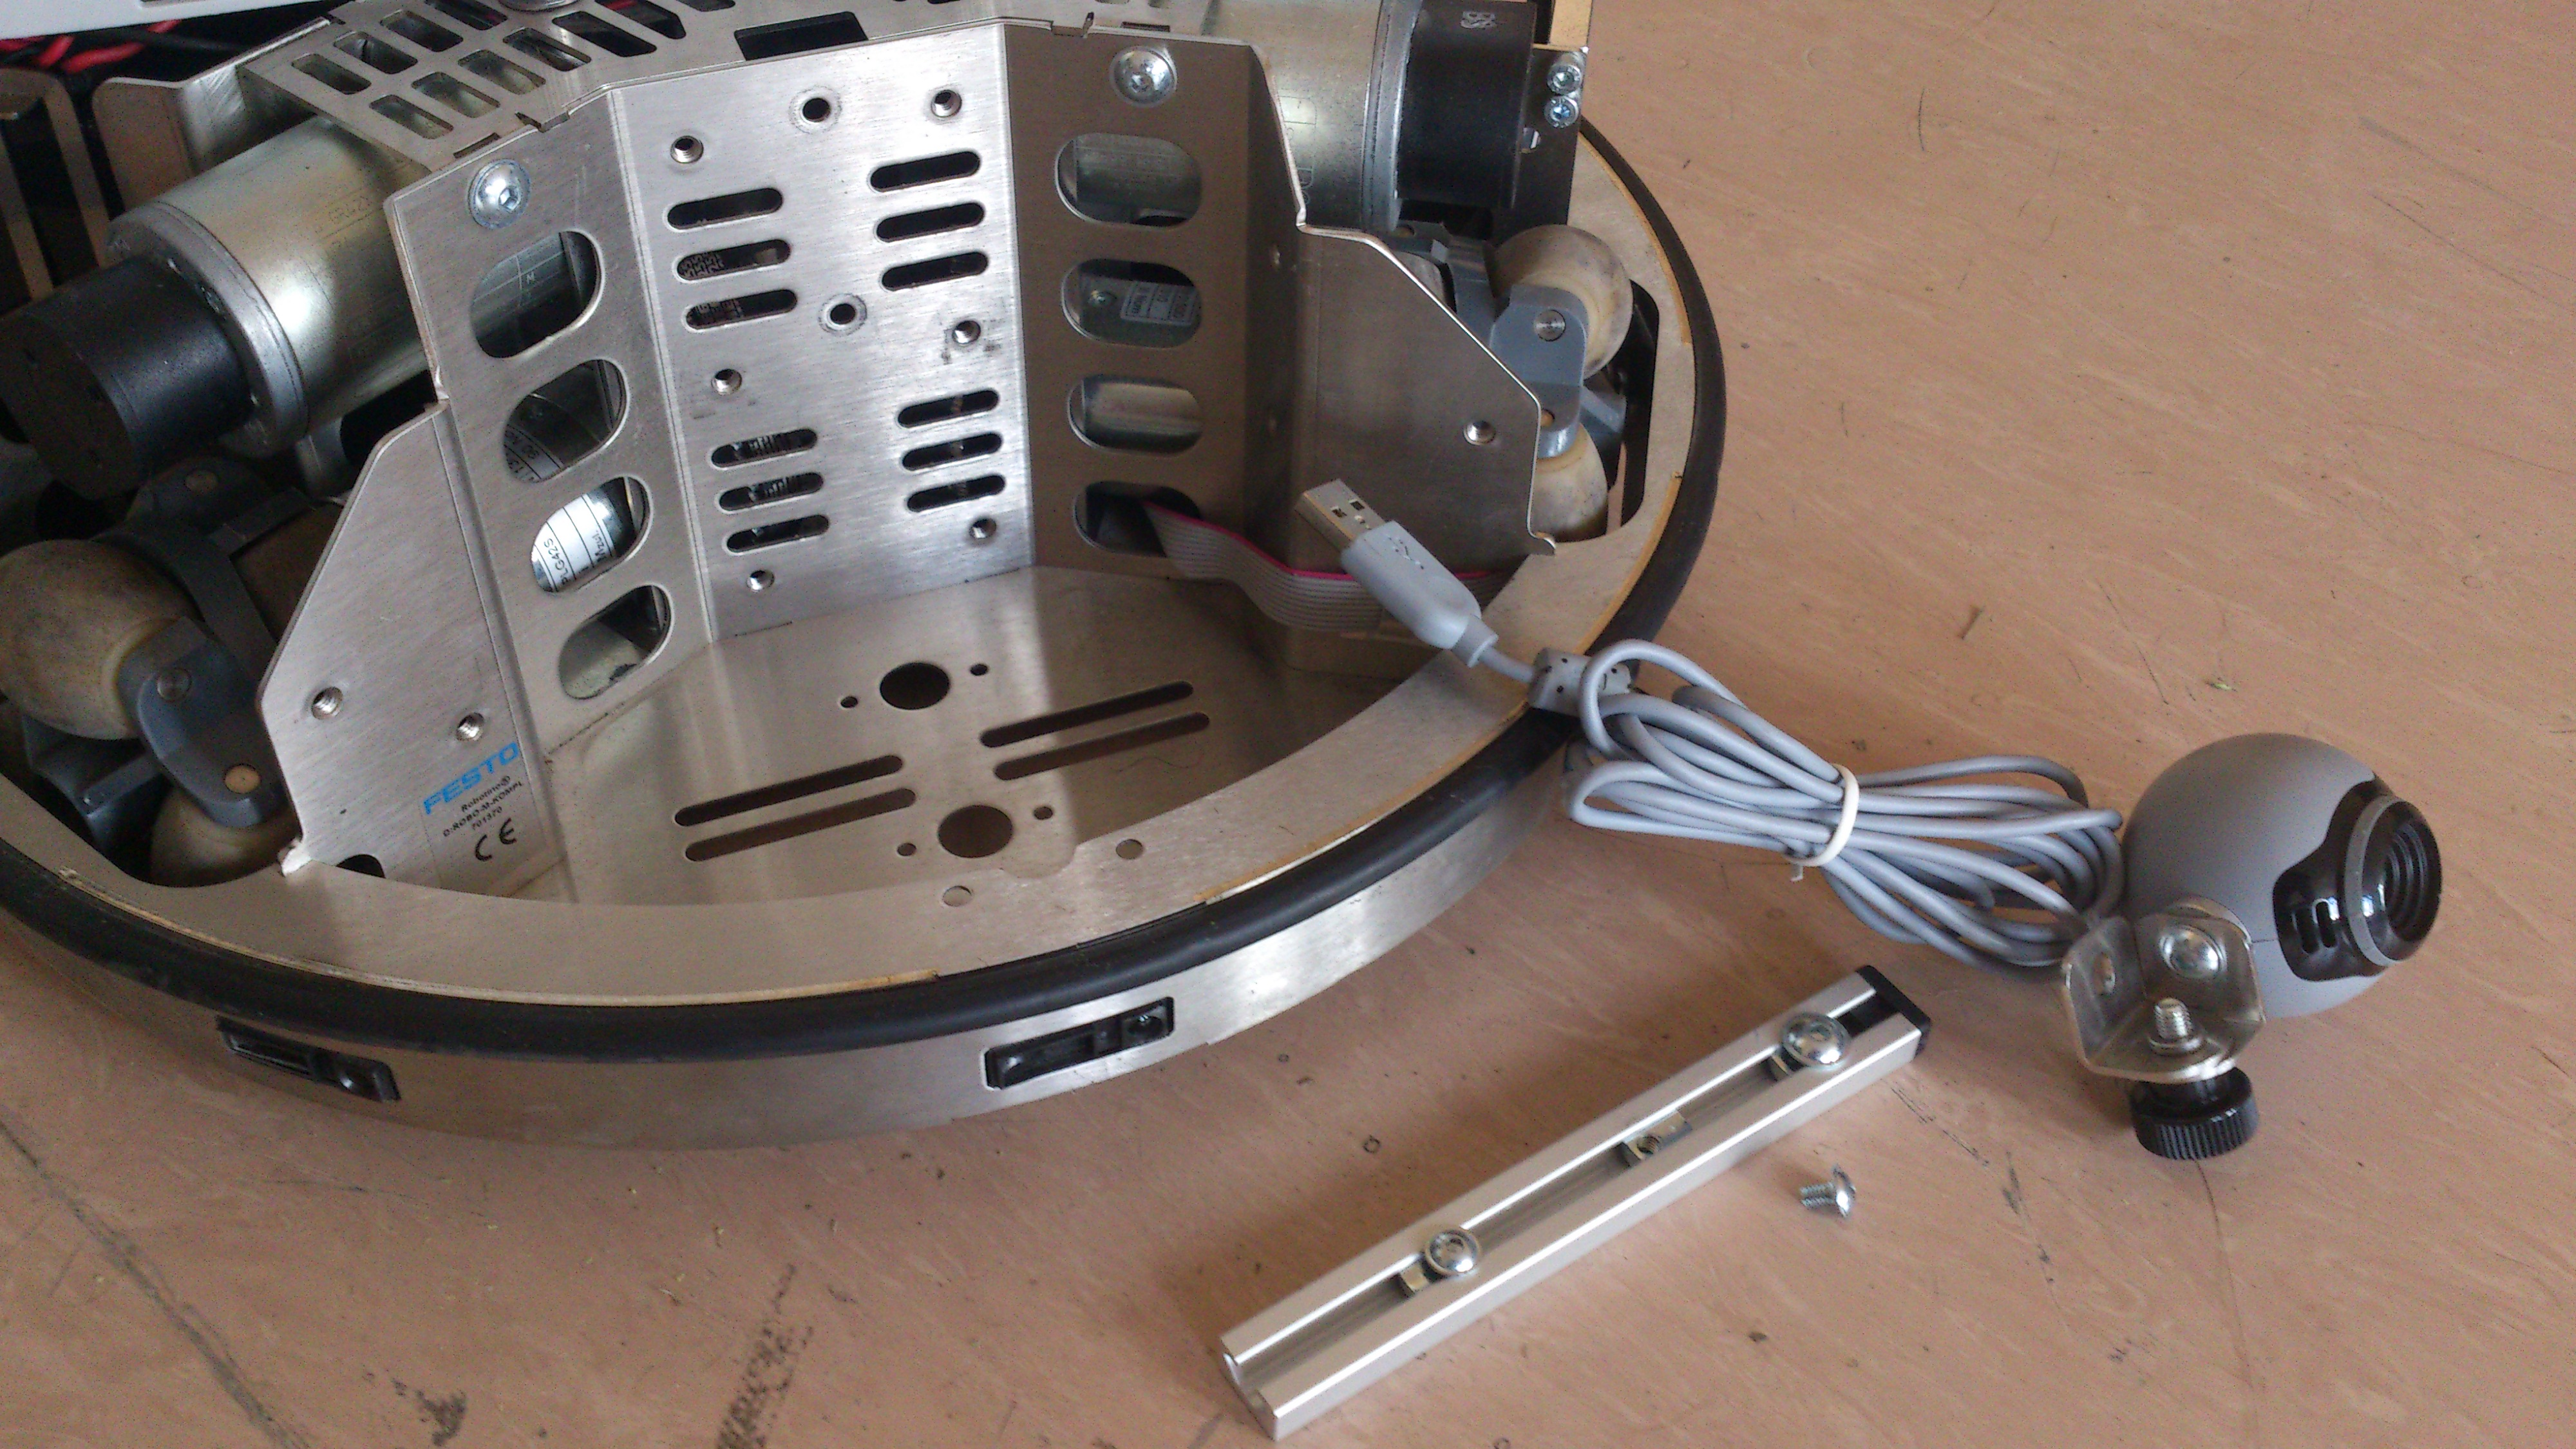
\includegraphics[height = 4.8cm]{web_cam_connection1.jpg} }
	\end{minipage}
	\hfill
	\begin{minipage}[h]{0.49\linewidth}
		\centering{ 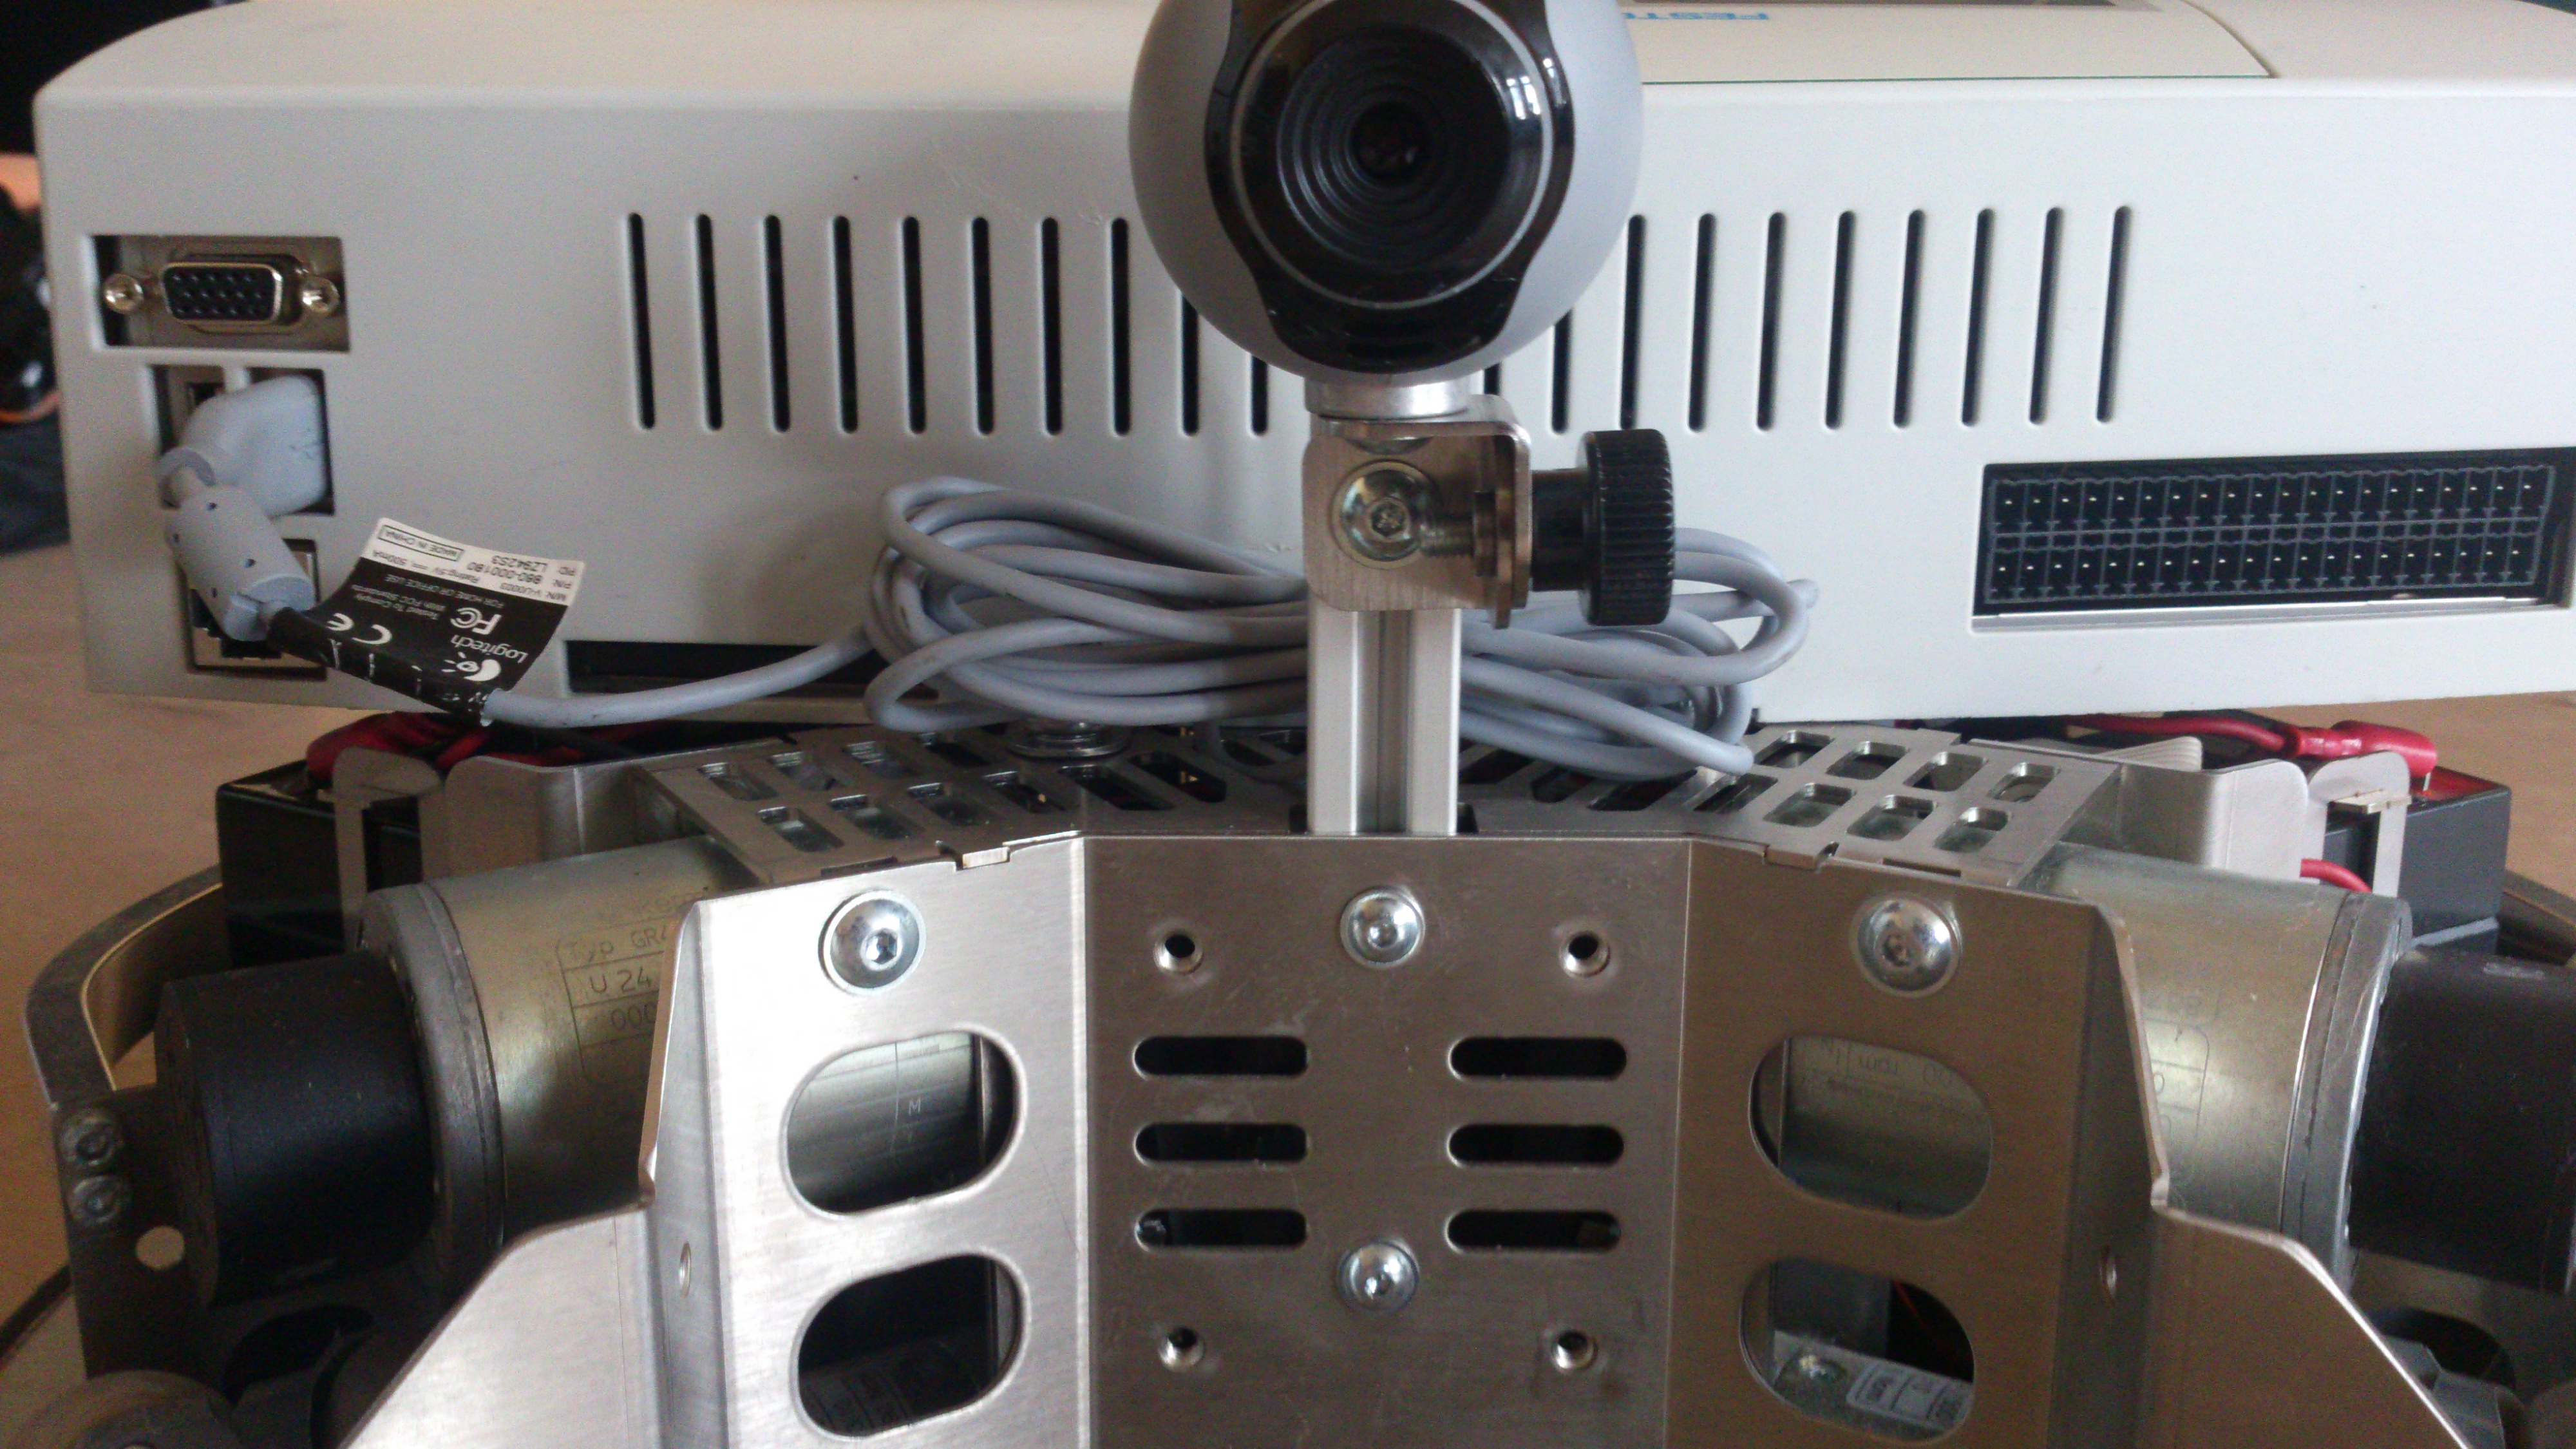
\includegraphics[height = 4.8cm]{web_cam_connection2.jpg} }
	\end{minipage}
	\caption{Монтаж вертикальной рейки на робота и установка на нее web-камеры.}
	\label{img_web_cam_connection}
\end{figure}



\subsection{Система NorthStar}
Система NorthStar~\cite{northstar_manual} предназначена для локализации Robotino в помещении.
Всего данная система состоит из устройств двух типов: проекторов и приемников.
Внешний вид последних можно видеть на рисунке~\ref{img_NSs_projector_and_receivers}.

\begin{figure}[h]
	\centering
	\includegraphics[height = 8cm]{ns_proj_receiv.png}
	\caption{Внешний вид составляющих частей системы NorthStar: 1~--- проекторов, 2~--- приемников.}
	\label{img_NSs_projector_and_receivers}
\end{figure}

Принцип работы данной системы состоит в том, что проектор излучает в инфракрасном диапазоне на потолок два световых пятна, а приемник по видимому изображению этих пятен на потолке определяет положение робота, на которого он установлен, относительно правосторонней системы координат, жестко связанной с проектором (обозначим ее как СКП).
При этом данная информация включает в себя не только сведения о координатах точки в СКП, в которой находится робот, но также и о его угле поворота относительно нее.
Точное положение самой СКП определяется из тех фактов, что ее начало находится в точке на полу, в которую проецируется середина отрезка, ограниченного на потолке упомянутыми выше световыми пятнами, а ось $OY$ лежит на прямой, проходящей через проекции с потолка на пол самих световых пятен.

Для определения положения на потолке инфракрасных пятен из-за их невидимости человеческому глазу разработчиками системы предусмотрена возможность их подсветки видимым красным светом (для иллюстрации к сказанному обратитесь к рисунку~\ref{img_NSs_coordinate_system}).
Для ее активации на несколько секунд достаточно коснуться пальцем металлизированного <<горла>> проектора.

\begin{figure}[h]
	\centering
	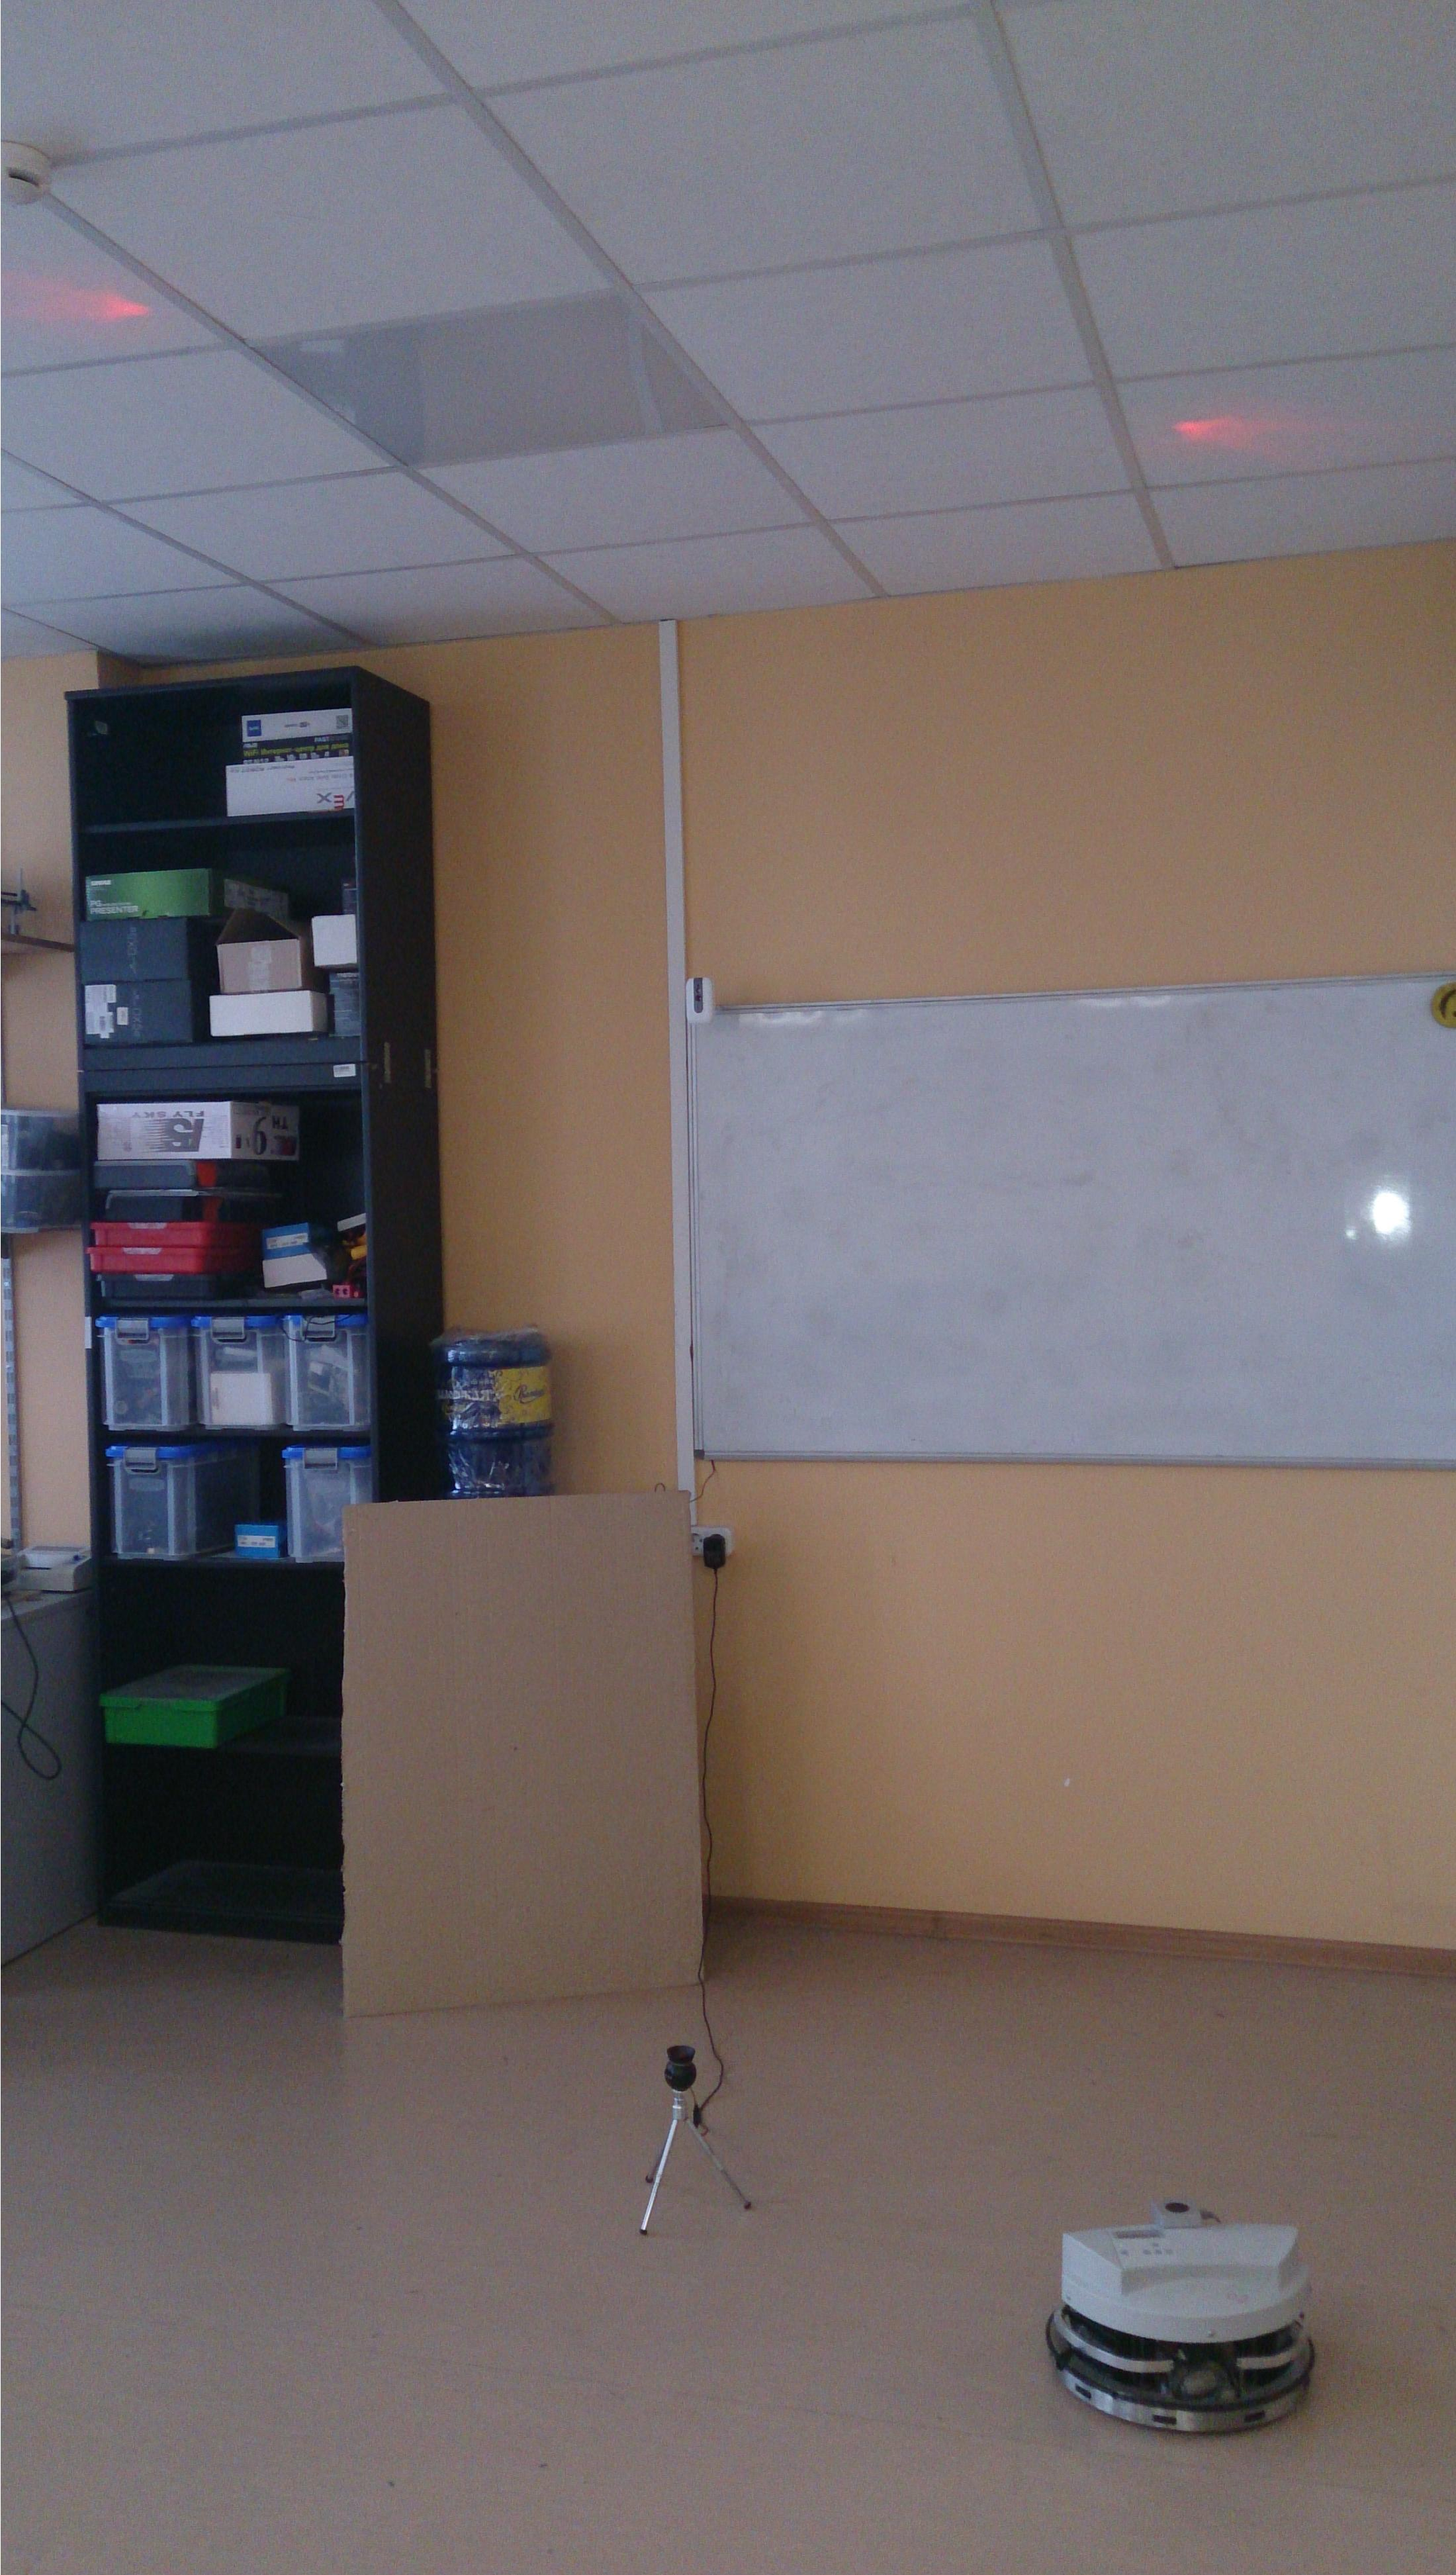
\includegraphics[height = 11cm]{ns_frame_and_red_dots.jpg}
	\caption{Система NorthStar в работе.}
	\label{img_NSs_coordinate_system}
\end{figure}

У~каждого проектора NorthStar на одной из его сторон есть переключатель набора частот, с которыми должны излучаться на потолок создаваемые им световые пятна (каждое пятно также проецируется с собственной, отдельной частотой).
Поскольку приемник способен различать частоты свечения пятен, то одновременно он может работать сразу с несколькими проекторами\lefteqn.\footnote{Для указания того, с каким проектором следует работать приемнику NorthStar, в относящемся к нему ПО используется параметр RoomId. Характер зависимости его значения от положения переключателя набора частот на проекторе показан в таблице из \cite[стр.~25]{northstar_manual}.}
Каждый проектор в свою очередь также может использоваться одновременно несколькими приемниками.

Для работы проектора достаточно подключить его к бытовой сети питания 220~В, для работы приемника~--- подключить его к роботу по USB.

Среди других эксплуатационных характеристик NortStar стоит выделить еще и то, что перед использованием данной системы в работе ее необходимо калибровать.
Конкретные действия, составляющие суть данного процесса, сводятся к тому, чтобы подобрать такое значение одного из входных параметров%
\footnote{В~дальнейшем он будет именоваться калибровочным коэффициентом. Официальная же документация к ПО робота приписывает ему значение высоты потолка~\cite{set_ceiling_cal_doc}.}
для управляющего работой приемника программного обеспечения, при котором смещение робота в жизни на расстояние в 1~м, будет соответствовать изменению в возвращаемых системой координатах, говорящему о том же~--- о смещении приемника в 1~м~\cite[стр.~30]{northstar_manual}.

Дополнительные сведения, касающиеся этой системы, можно узнать в Приложении~\ref{app_about_ns}.



\subsection{Подключение лидара}
Лидар (Laser range finder) Hokuyo URG-04LX-UG01 представляет собой датчик, который сканирует одну плоскость окружающего его пространства и определяет в ней расстояния, отделяющие его от препятствий (см.~рисунок~\ref{img_lidar_at_work}).
Эти расстояния относятся к направлениям, описываемым некоторым множеством углов.
Например, последнее для этого датчика может быть равным $[-120^\circ, -119.64^\circ, -119.28^\circ, \ldots, 120^\circ]$ (подразумевается, что угол~$0^\circ$ соответствует направлению <<вперед>> относительно лидара).
Согласно паспорту (см.~datasheet в~\cite{lidar}), датчик способен фиксировать препятствия, находящиеся от него на расстоянии от 20 мм до 5600 мм, однако опыт его использования показывает, что предметы, удаленные от него больше, чем на 3 метра, стабильно могут не детектироваться.

\begin{figure}[h!]
	\centering
	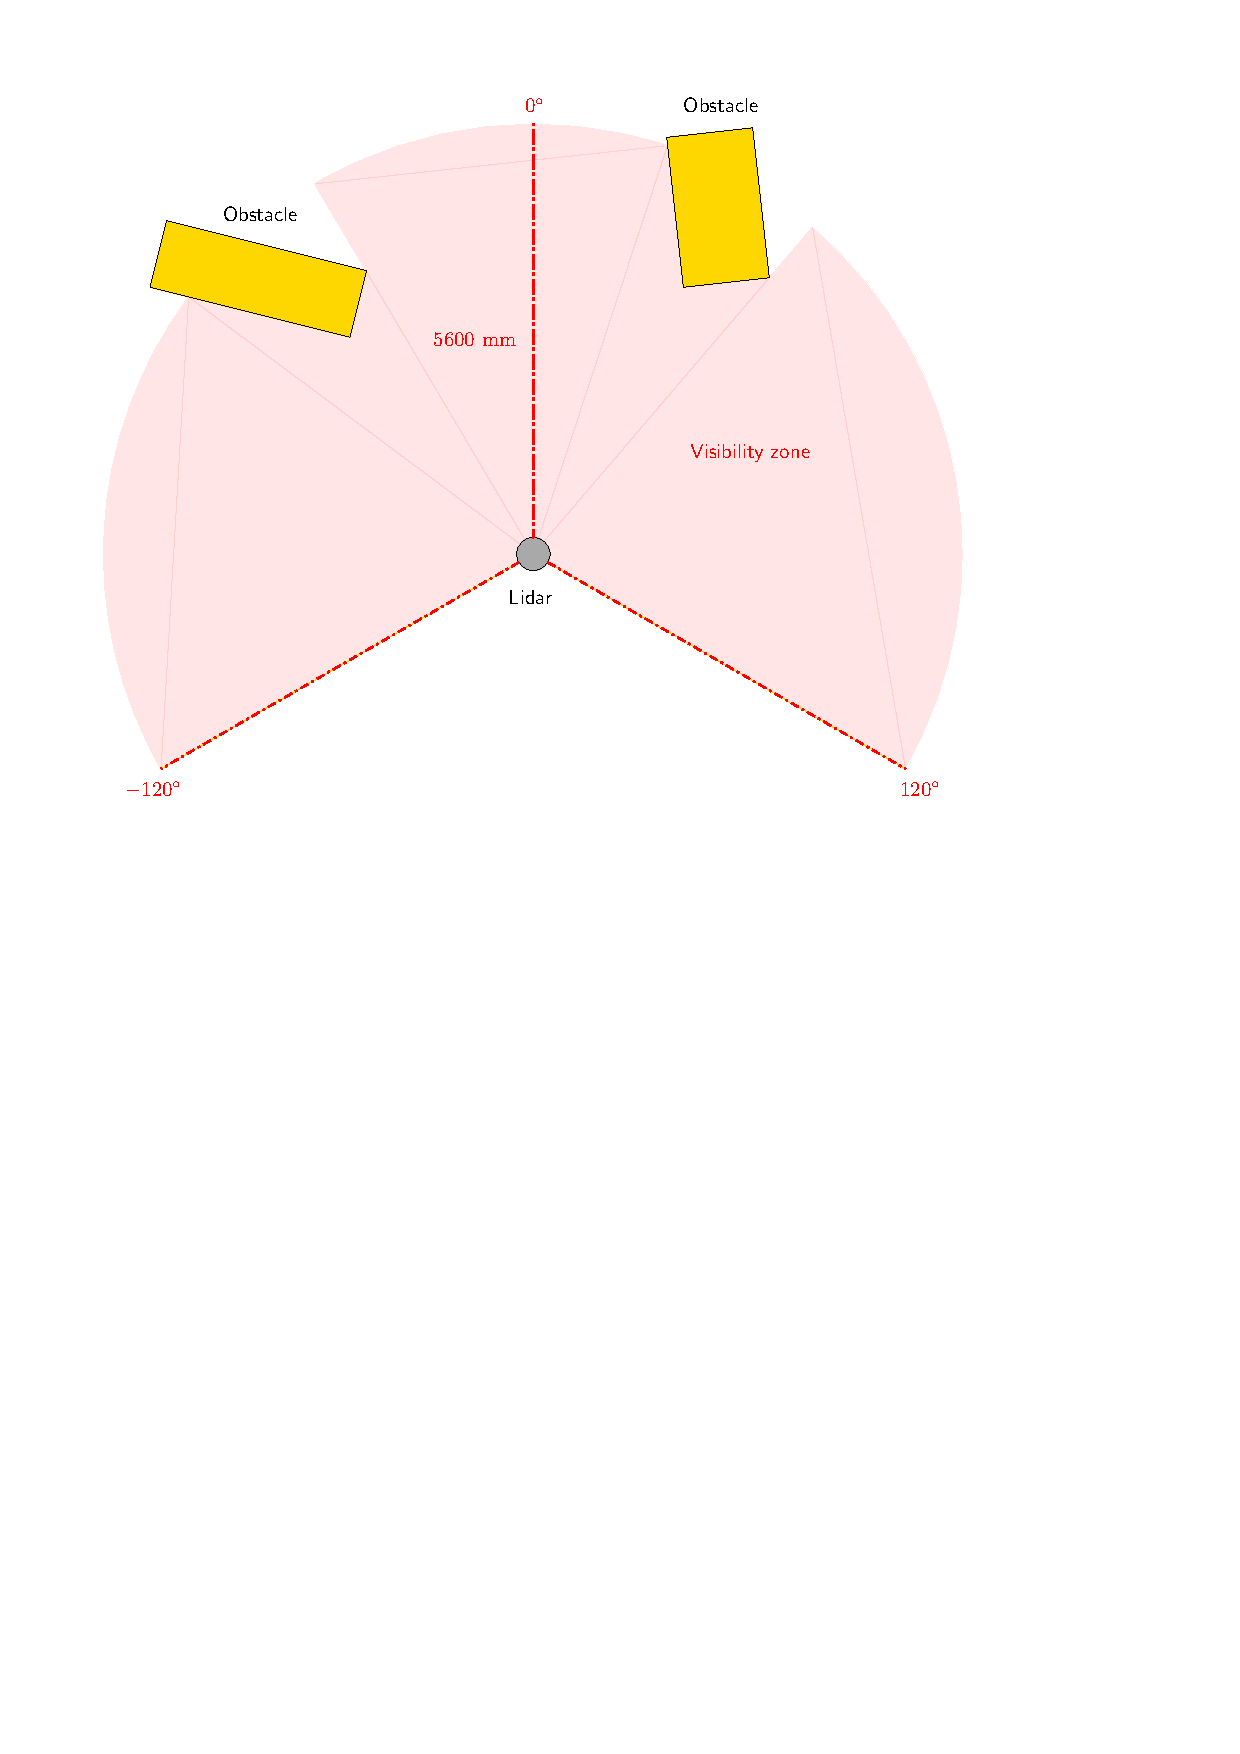
\includegraphics[width=0.55\textwidth]{lidar_at_work.pdf}
	\caption{Лидар в работе (схема; вид сверху).}
	\label{img_lidar_at_work}
\end{figure}

Для подключения лидара к Robotino вставьте в USB-порты оба свободных конца его Y-образного кабеля (см.~рисунок~\ref{img_lidar_connection}).
Ограничиваться подключением к роботу только одного из концов категорически запрещено, так как это может привести к поломке как самого робота, так и датчика.
Дело в том, что для работы последнего требуется ток, который может превышать 500~мА~--- максимальное значение для выходного тока одного USB-порта.

\begin{figure}[h!]
	\centering
	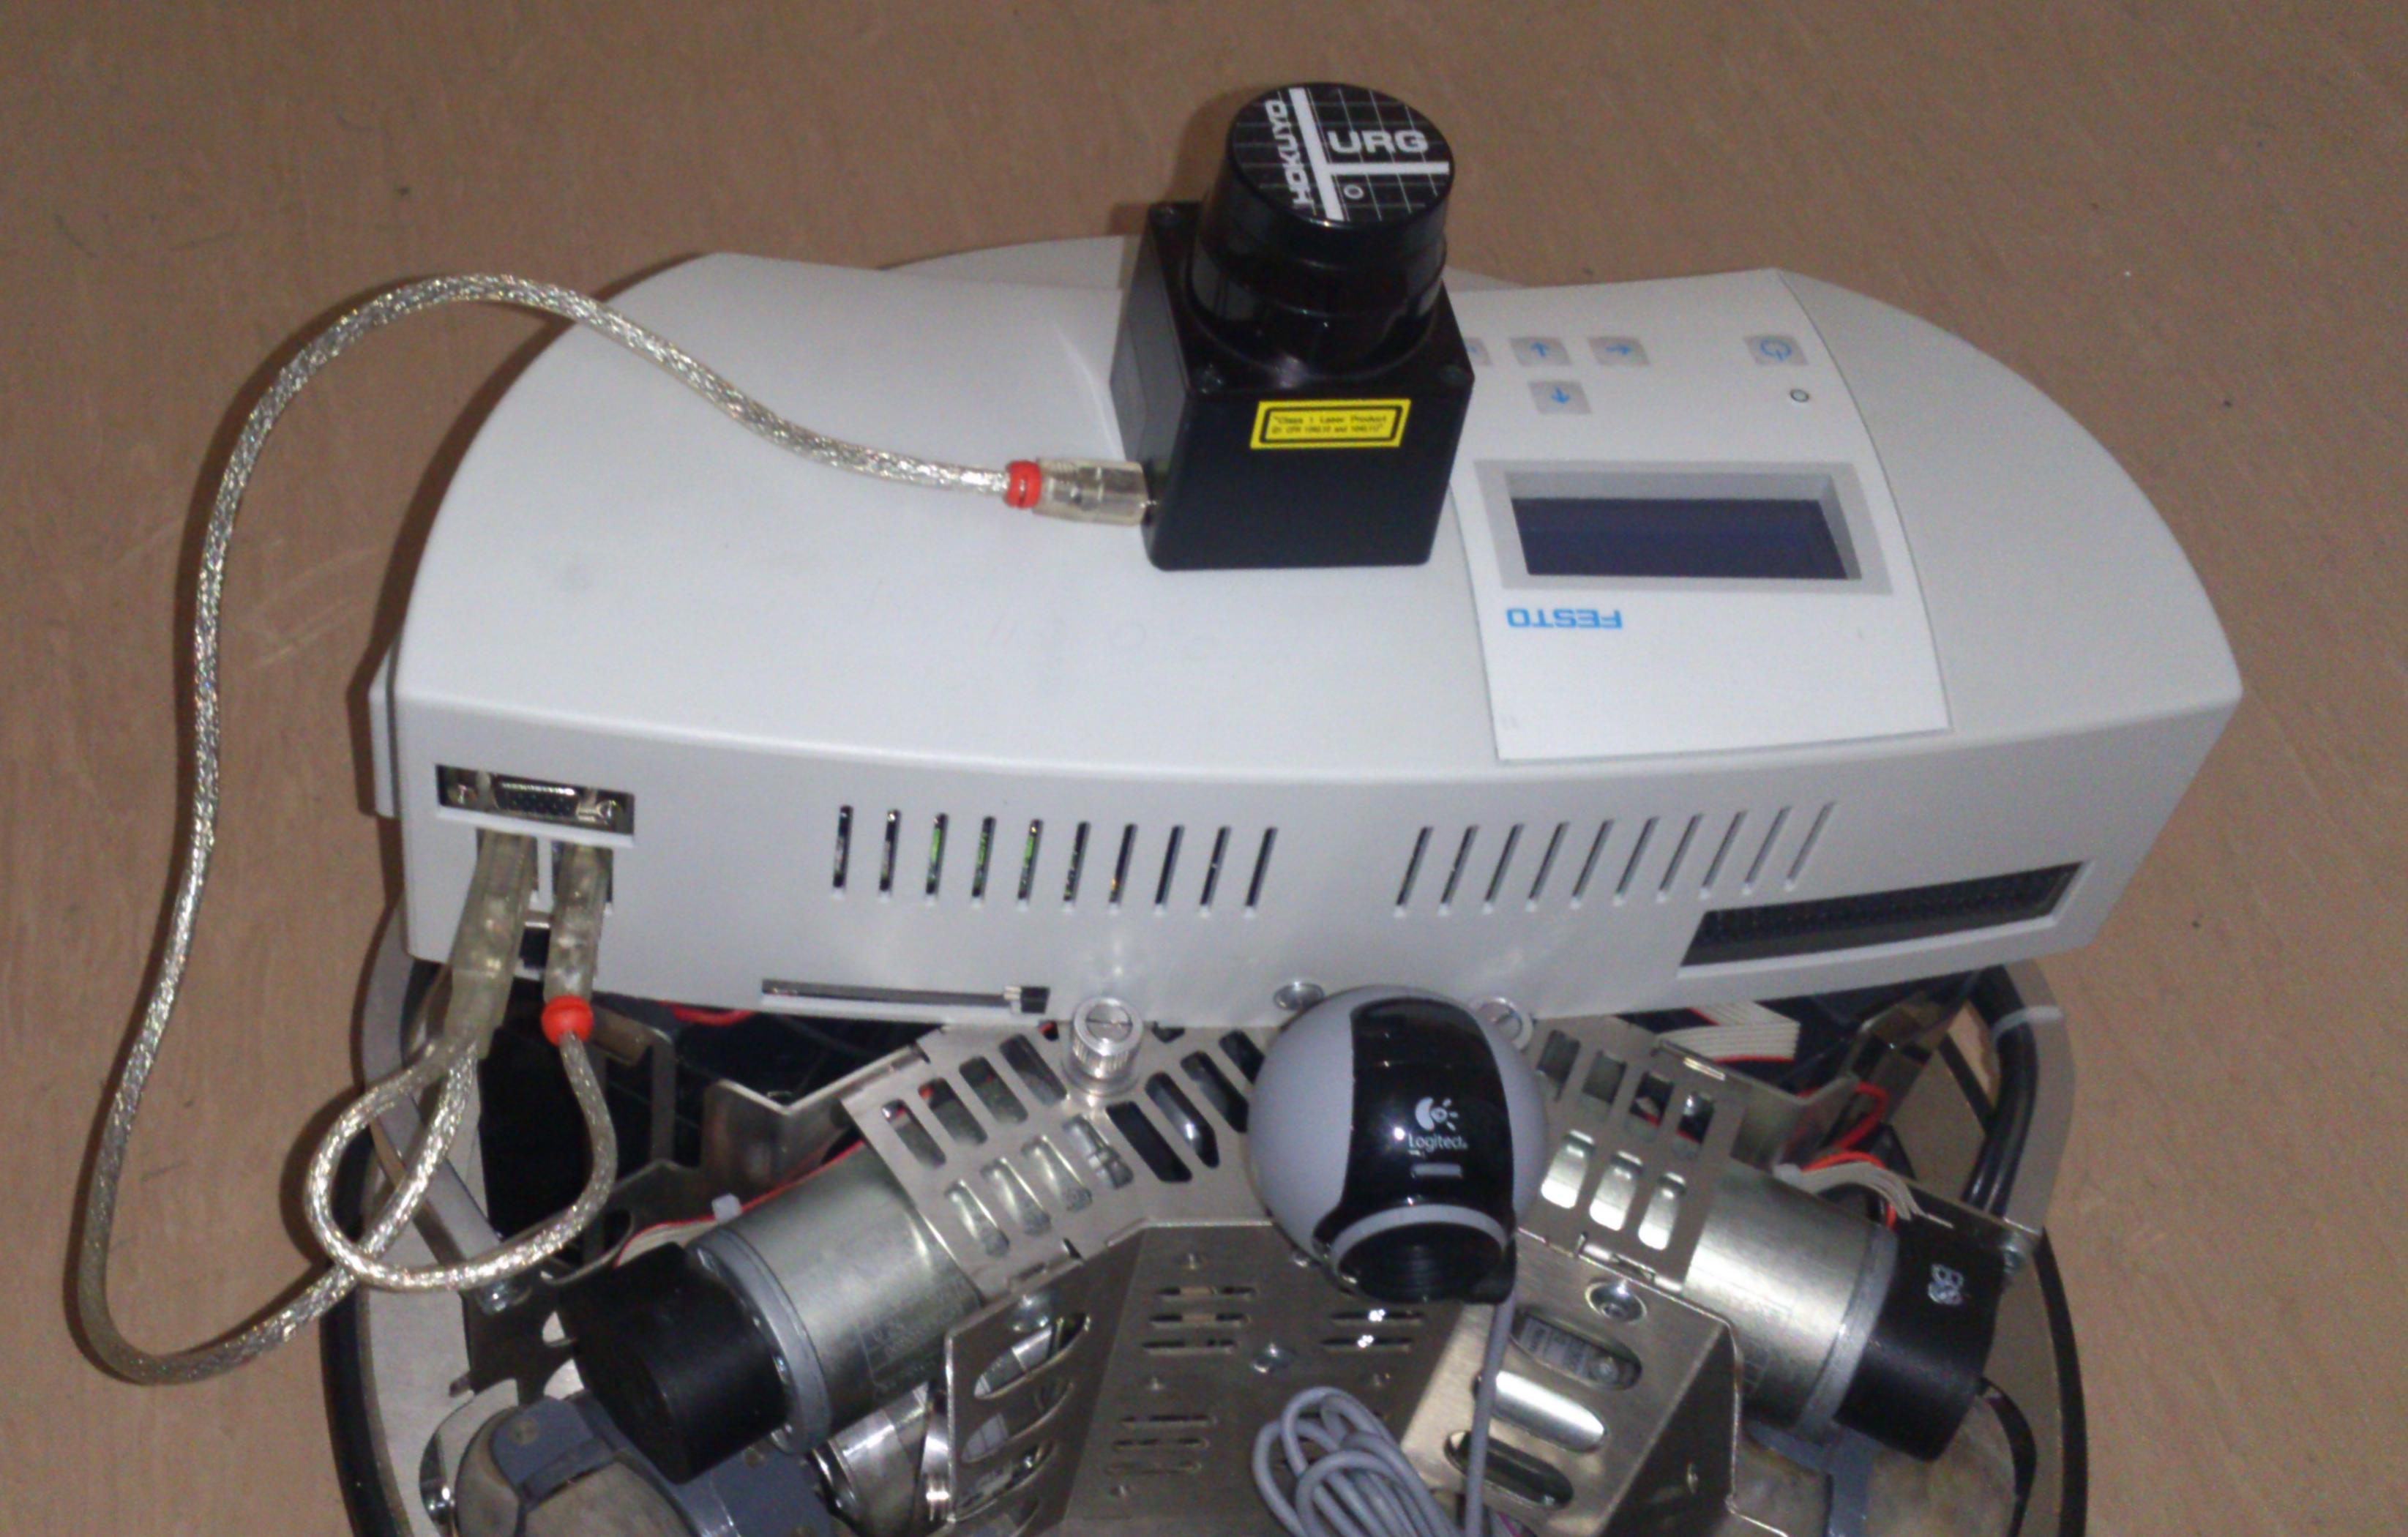
\includegraphics[width=0.65\textwidth]{lidar_connection.jpg}
	\caption{Подключение лидара к роботу.}
	\label{img_lidar_connection}
\end{figure}



\subsection{Подключение датчика-металлоискателя (inductive sensor)}
Металлоискатель (см.~рисунок~\ref{img_inductive}) представляет собой датчик, который возвращает аналоговый сигнал, числовое значение которого тем меньше, чем ближе к сенсору находится какой-либо металлический объект.
При этом дальность действия датчика составляет всего 6~мм.

\begin{figure}[h!]
	\centering
	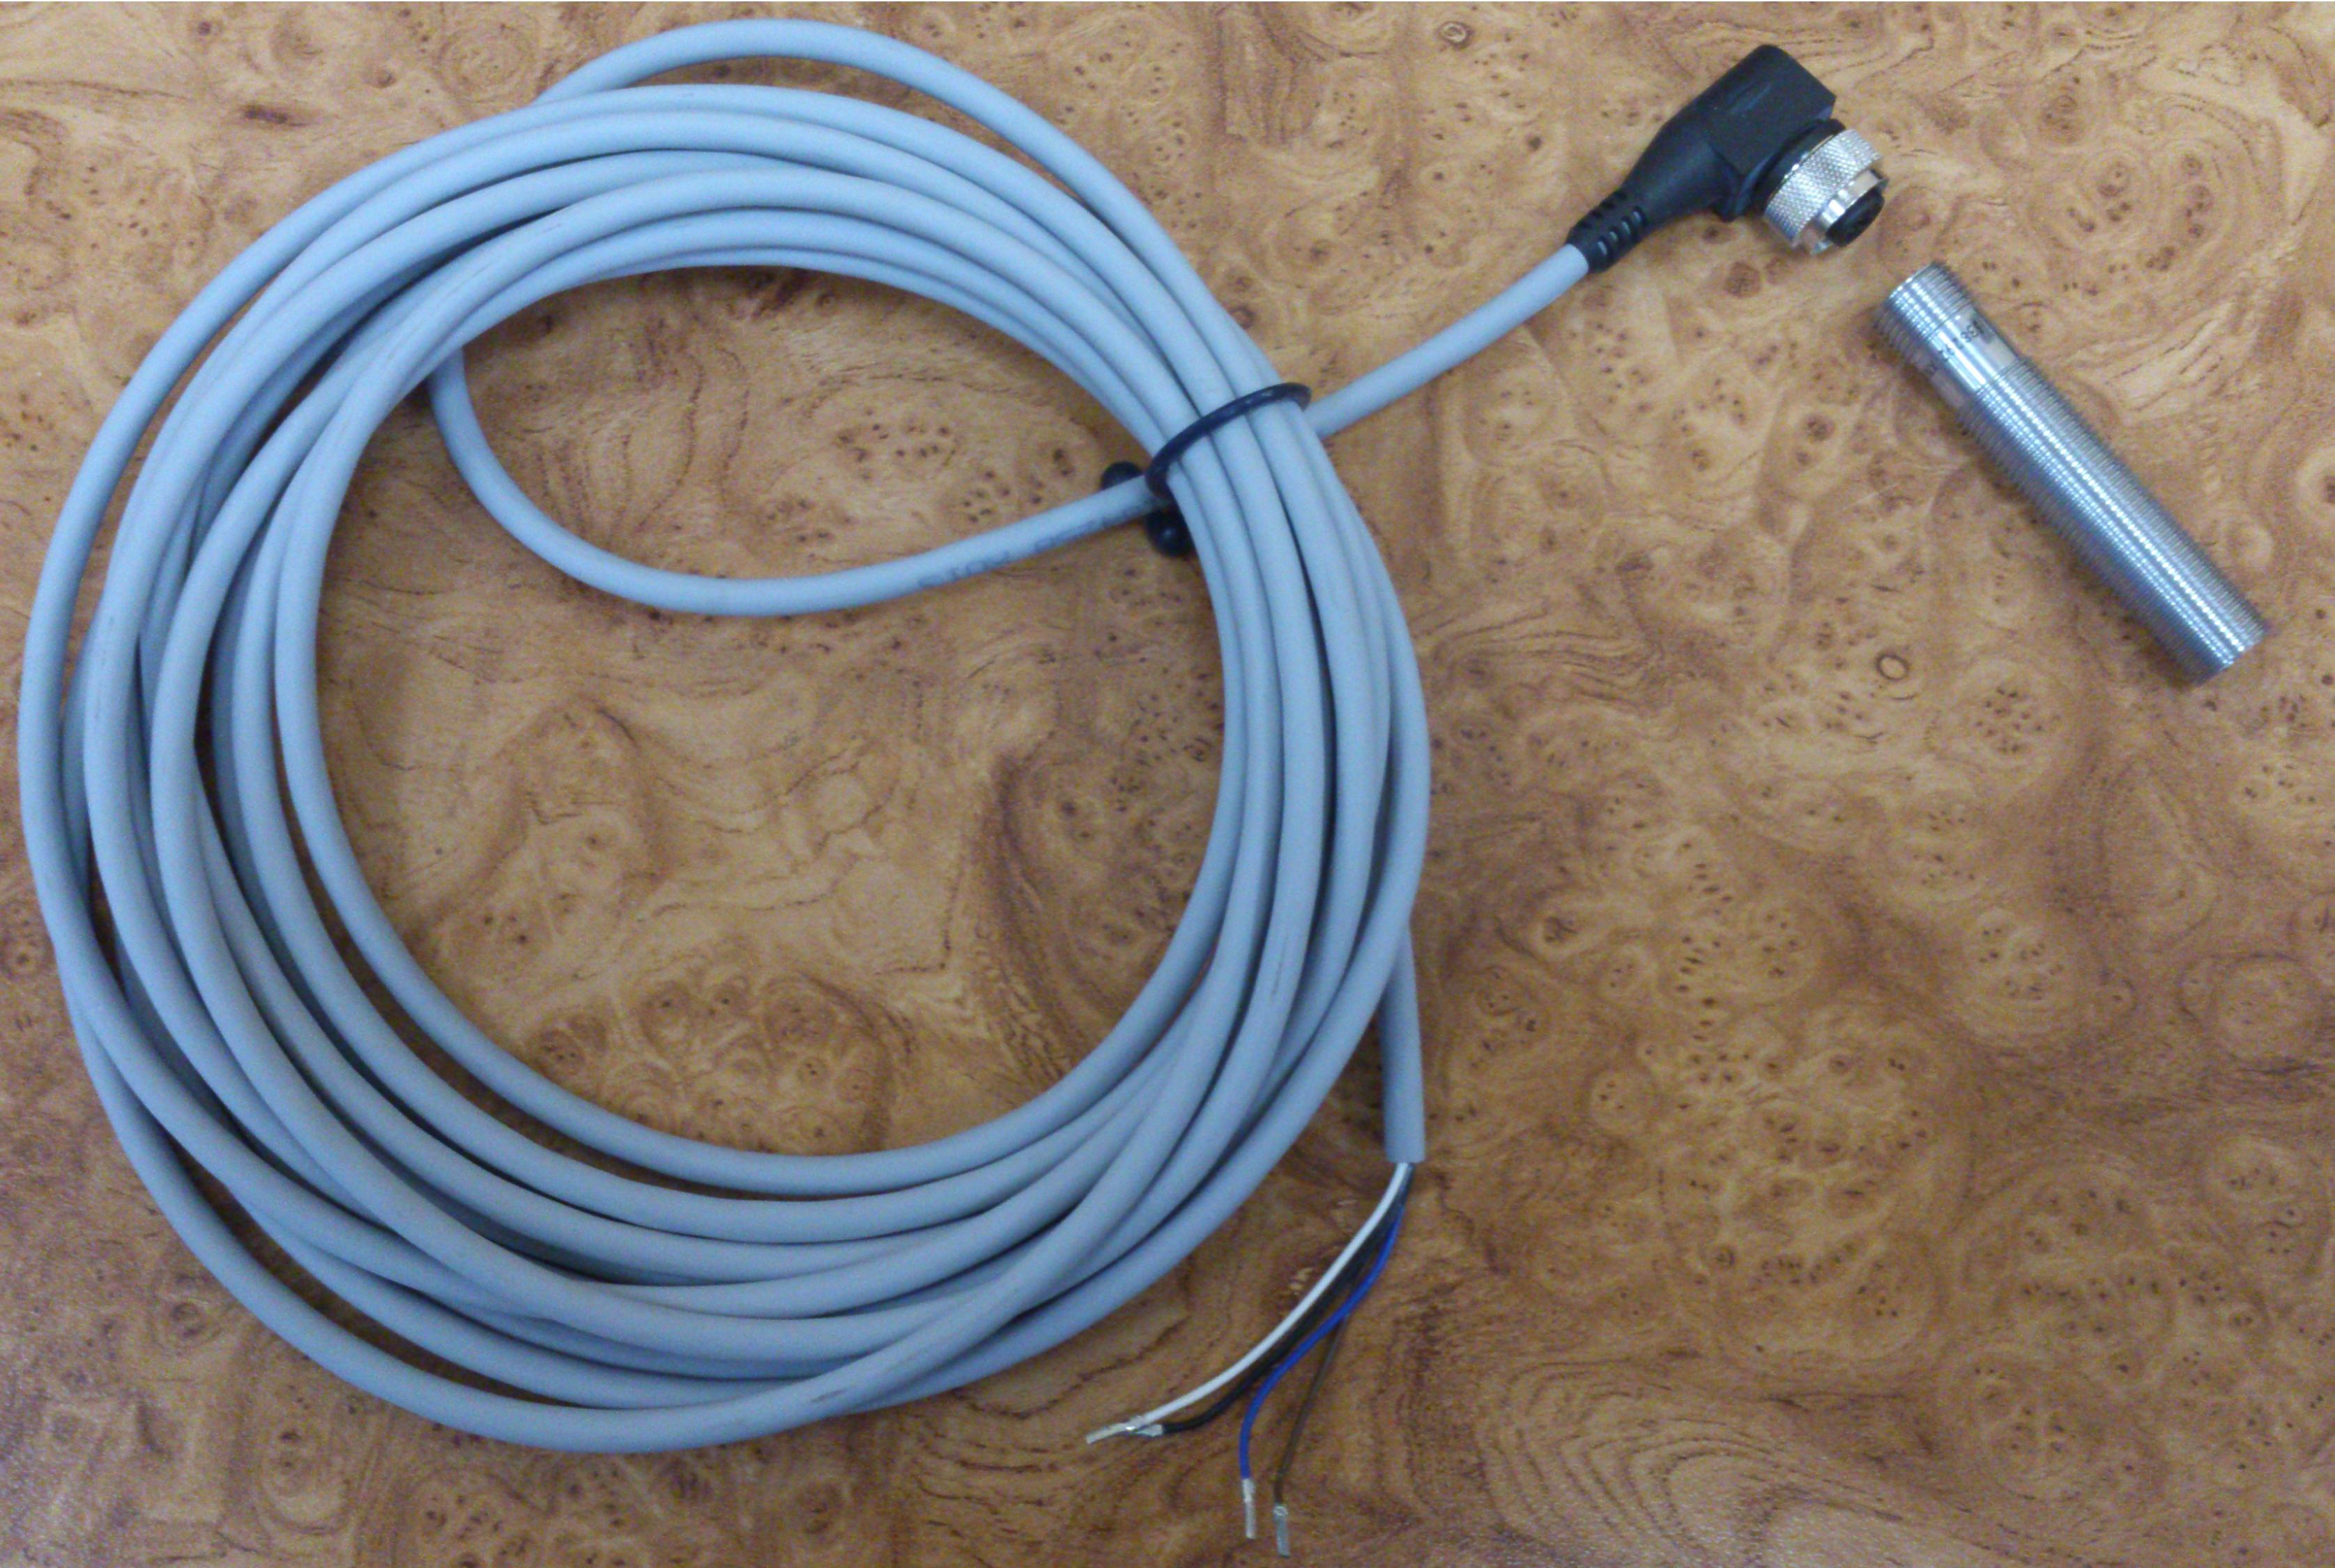
\includegraphics[width=0.65\textwidth]{inductive.jpg}
	\caption{Датчик-металлоискатель и кабель, с помощью которого он подключается.}
	\label{img_inductive}
\end{figure}

Для электрического подключения этого датчика к Robotino (см.~стр.~30 руководства с~\cite{news_manual}) воткните коричневый провод датчика в любое гнездо клеммника, соответствующее порту с названием «24V», синий провод – в любое гнездо клеммника, соответствующее порту с названием «GND», а черный~--- в любое гнездо клеммника, соответствующее порту с названием «AIN?», где ?~--- одно из чисел, составляющих множество $[1, 2, \ldots, 8]$.
Белый провод оставьте неподключенным (см.~рисунок~\ref{img_inductive_connect}).

\begin{figure}[h!]
	\centering
	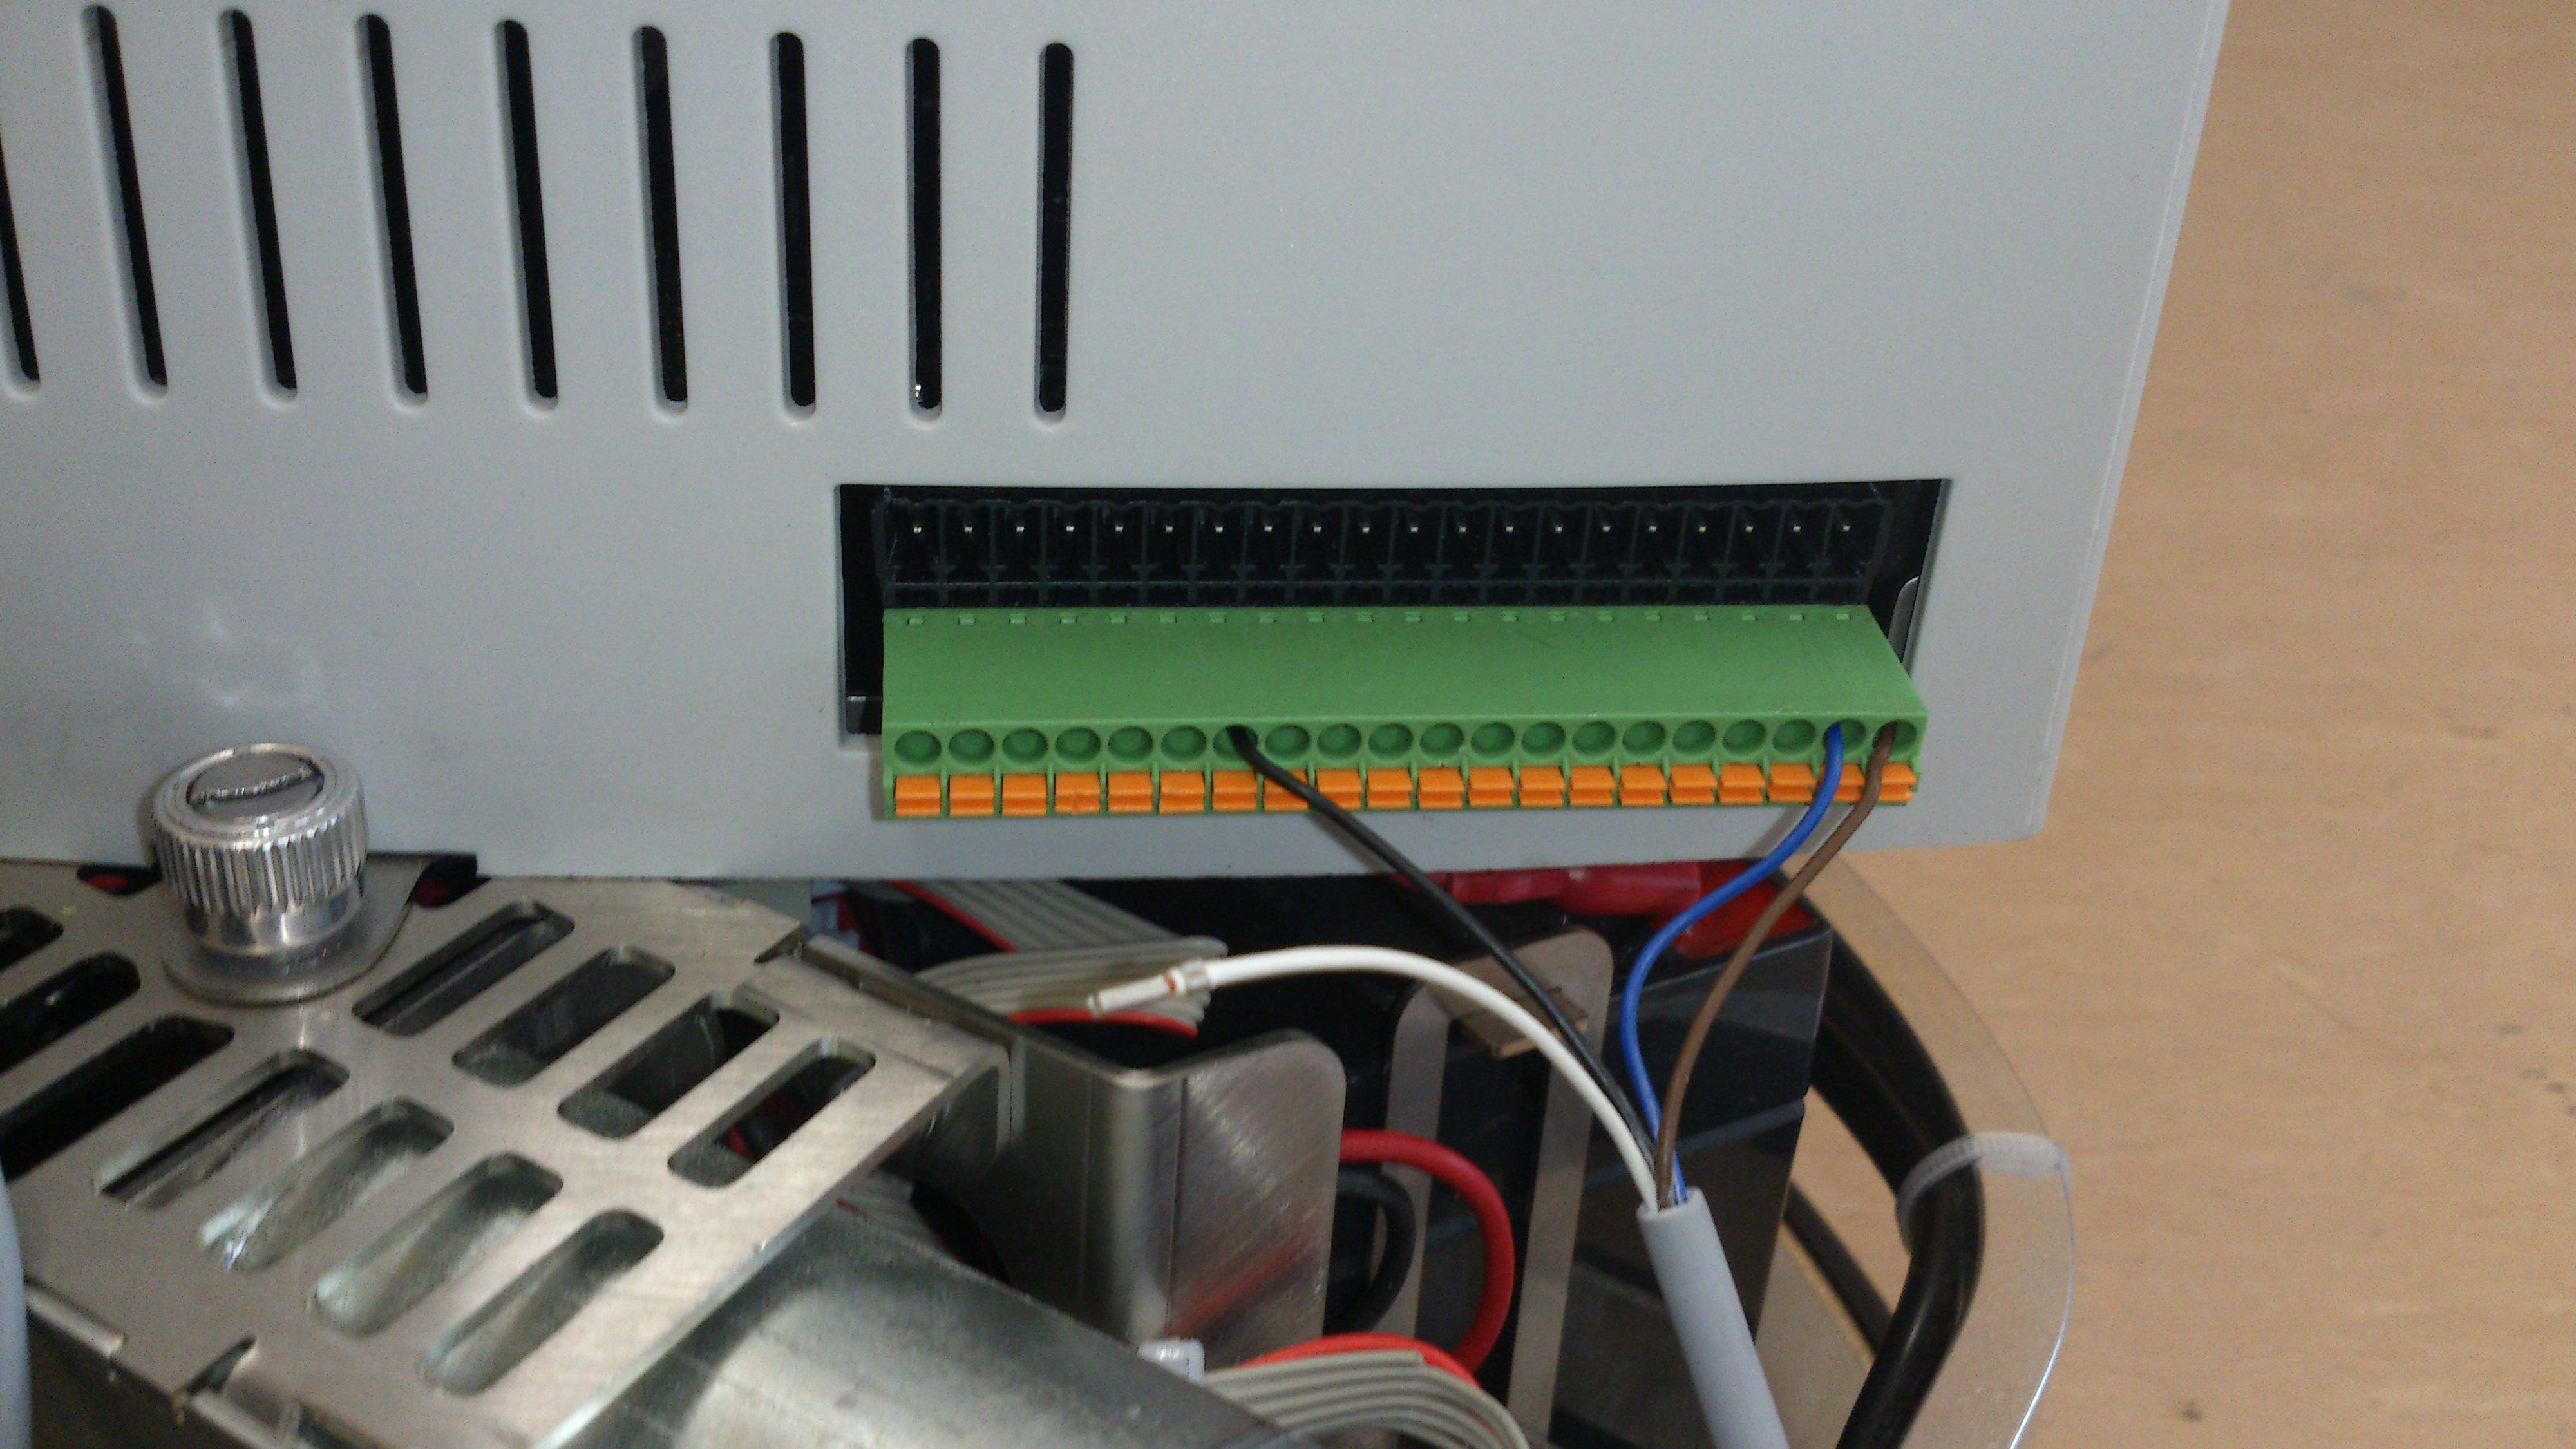
\includegraphics[width=0.65\textwidth]{inductive_connect.jpg}
	\caption{Пример подключения проводов кабеля датчика-металлоискателя.}
	\label{img_inductive_connect}
\end{figure}

Для механического монтажа данного датчика производителем предусмотрены несколько отверстий в колесной платформе Robotino.
Способ крепления выберите по вкусу.
При этом учтите, что в руководстве пользователя от Robotino более поздней модели рекомендуется просто зафиксировать датчик в желаемом положении с помощью двух гаек~\cite{news_manual}, а на сайте производителя встречаются такие сборочные единицы с участием этого датчика, как \cite{strange1, strange2}.



\subsection{Подключение оптического датчика (Opto-electronic sensors)}
Оптические датчики (см.~рисунок~\ref{img_optical}) можно использовать для решения двух задач.
Во-первых, с их помощью можно определять цвет интересующей поверхности, однако только с точностью до <<белая она или черная>>.
Во-вторых, их можно использовать в качестве световых барьеров~--- датчиков, изменяющих состояние своего выходного сигнала при пересечении каким-либо объектом прямой линии, соединяющей излучатель и приемник (пример применения оптических датчиков в этой роли~--- см.~подраздел~\ref{part_gripper_connect}).

\begin{figure}[h!]
	\centering
	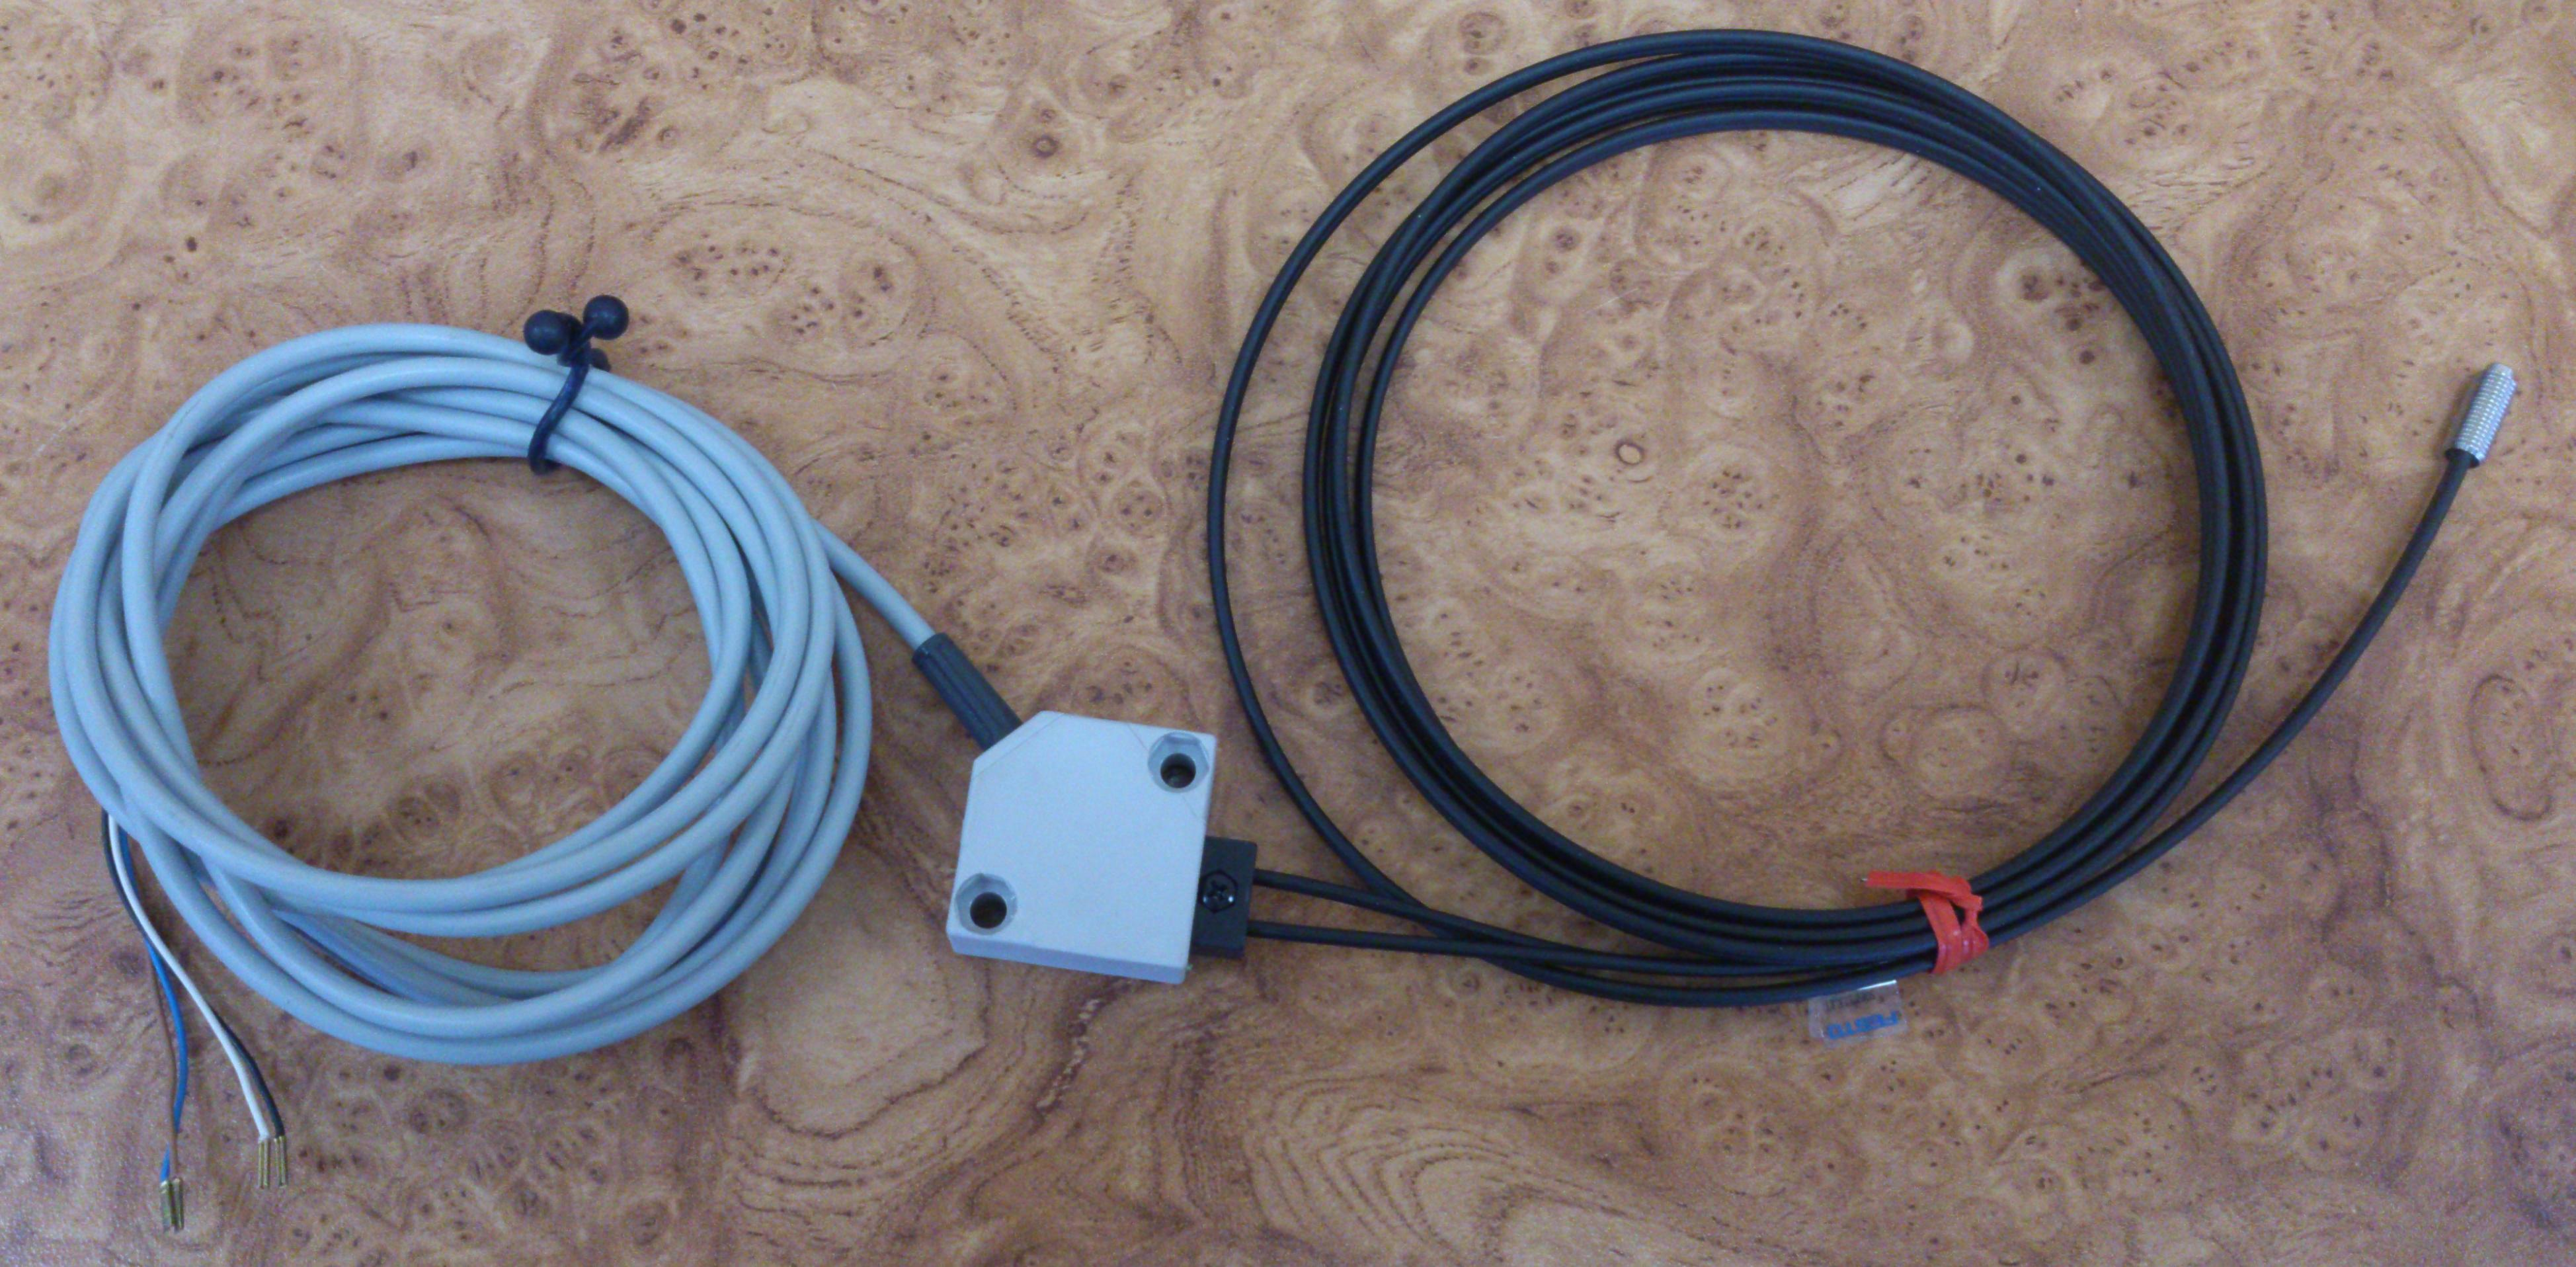
\includegraphics[width=0.65\textwidth]{optical.jpg}
	\caption{Оптический датчик с подключенным к нему сдвоенным световодом.}
	\label{img_optical}
\end{figure}

Для электрического подключения этого сенсора к Robotino (см.~стр.~28--30 руководства с~\cite{news_manual}) подключите его коричневый провод к любому из портов под названием «24V», синий~--- к любому из портов под названием «GND», а белый и черный~--- к любым двум из портов под названиями «DI?», где ?~--- одно значение из множества $[1, 2, \ldots, 8]$.
Цифровые сигналы, передаваемые с помощью белого и черного проводов являются инвертированными по отношению друг к другу, следовательно можно ограничиться подключением либо только белого, либо только черного провода.

Для крепления оптических датчиков у Robotino специально предусмотрено несколько посадочных мест (см.~рисунки~\ref{img_optical_connect} и~\ref{img_gripper_with_barrier}).
При этом в качестве крепежных элементов подразумевается использовать две пары болт-гайка.

\begin{figure}[h!]
	\centering
	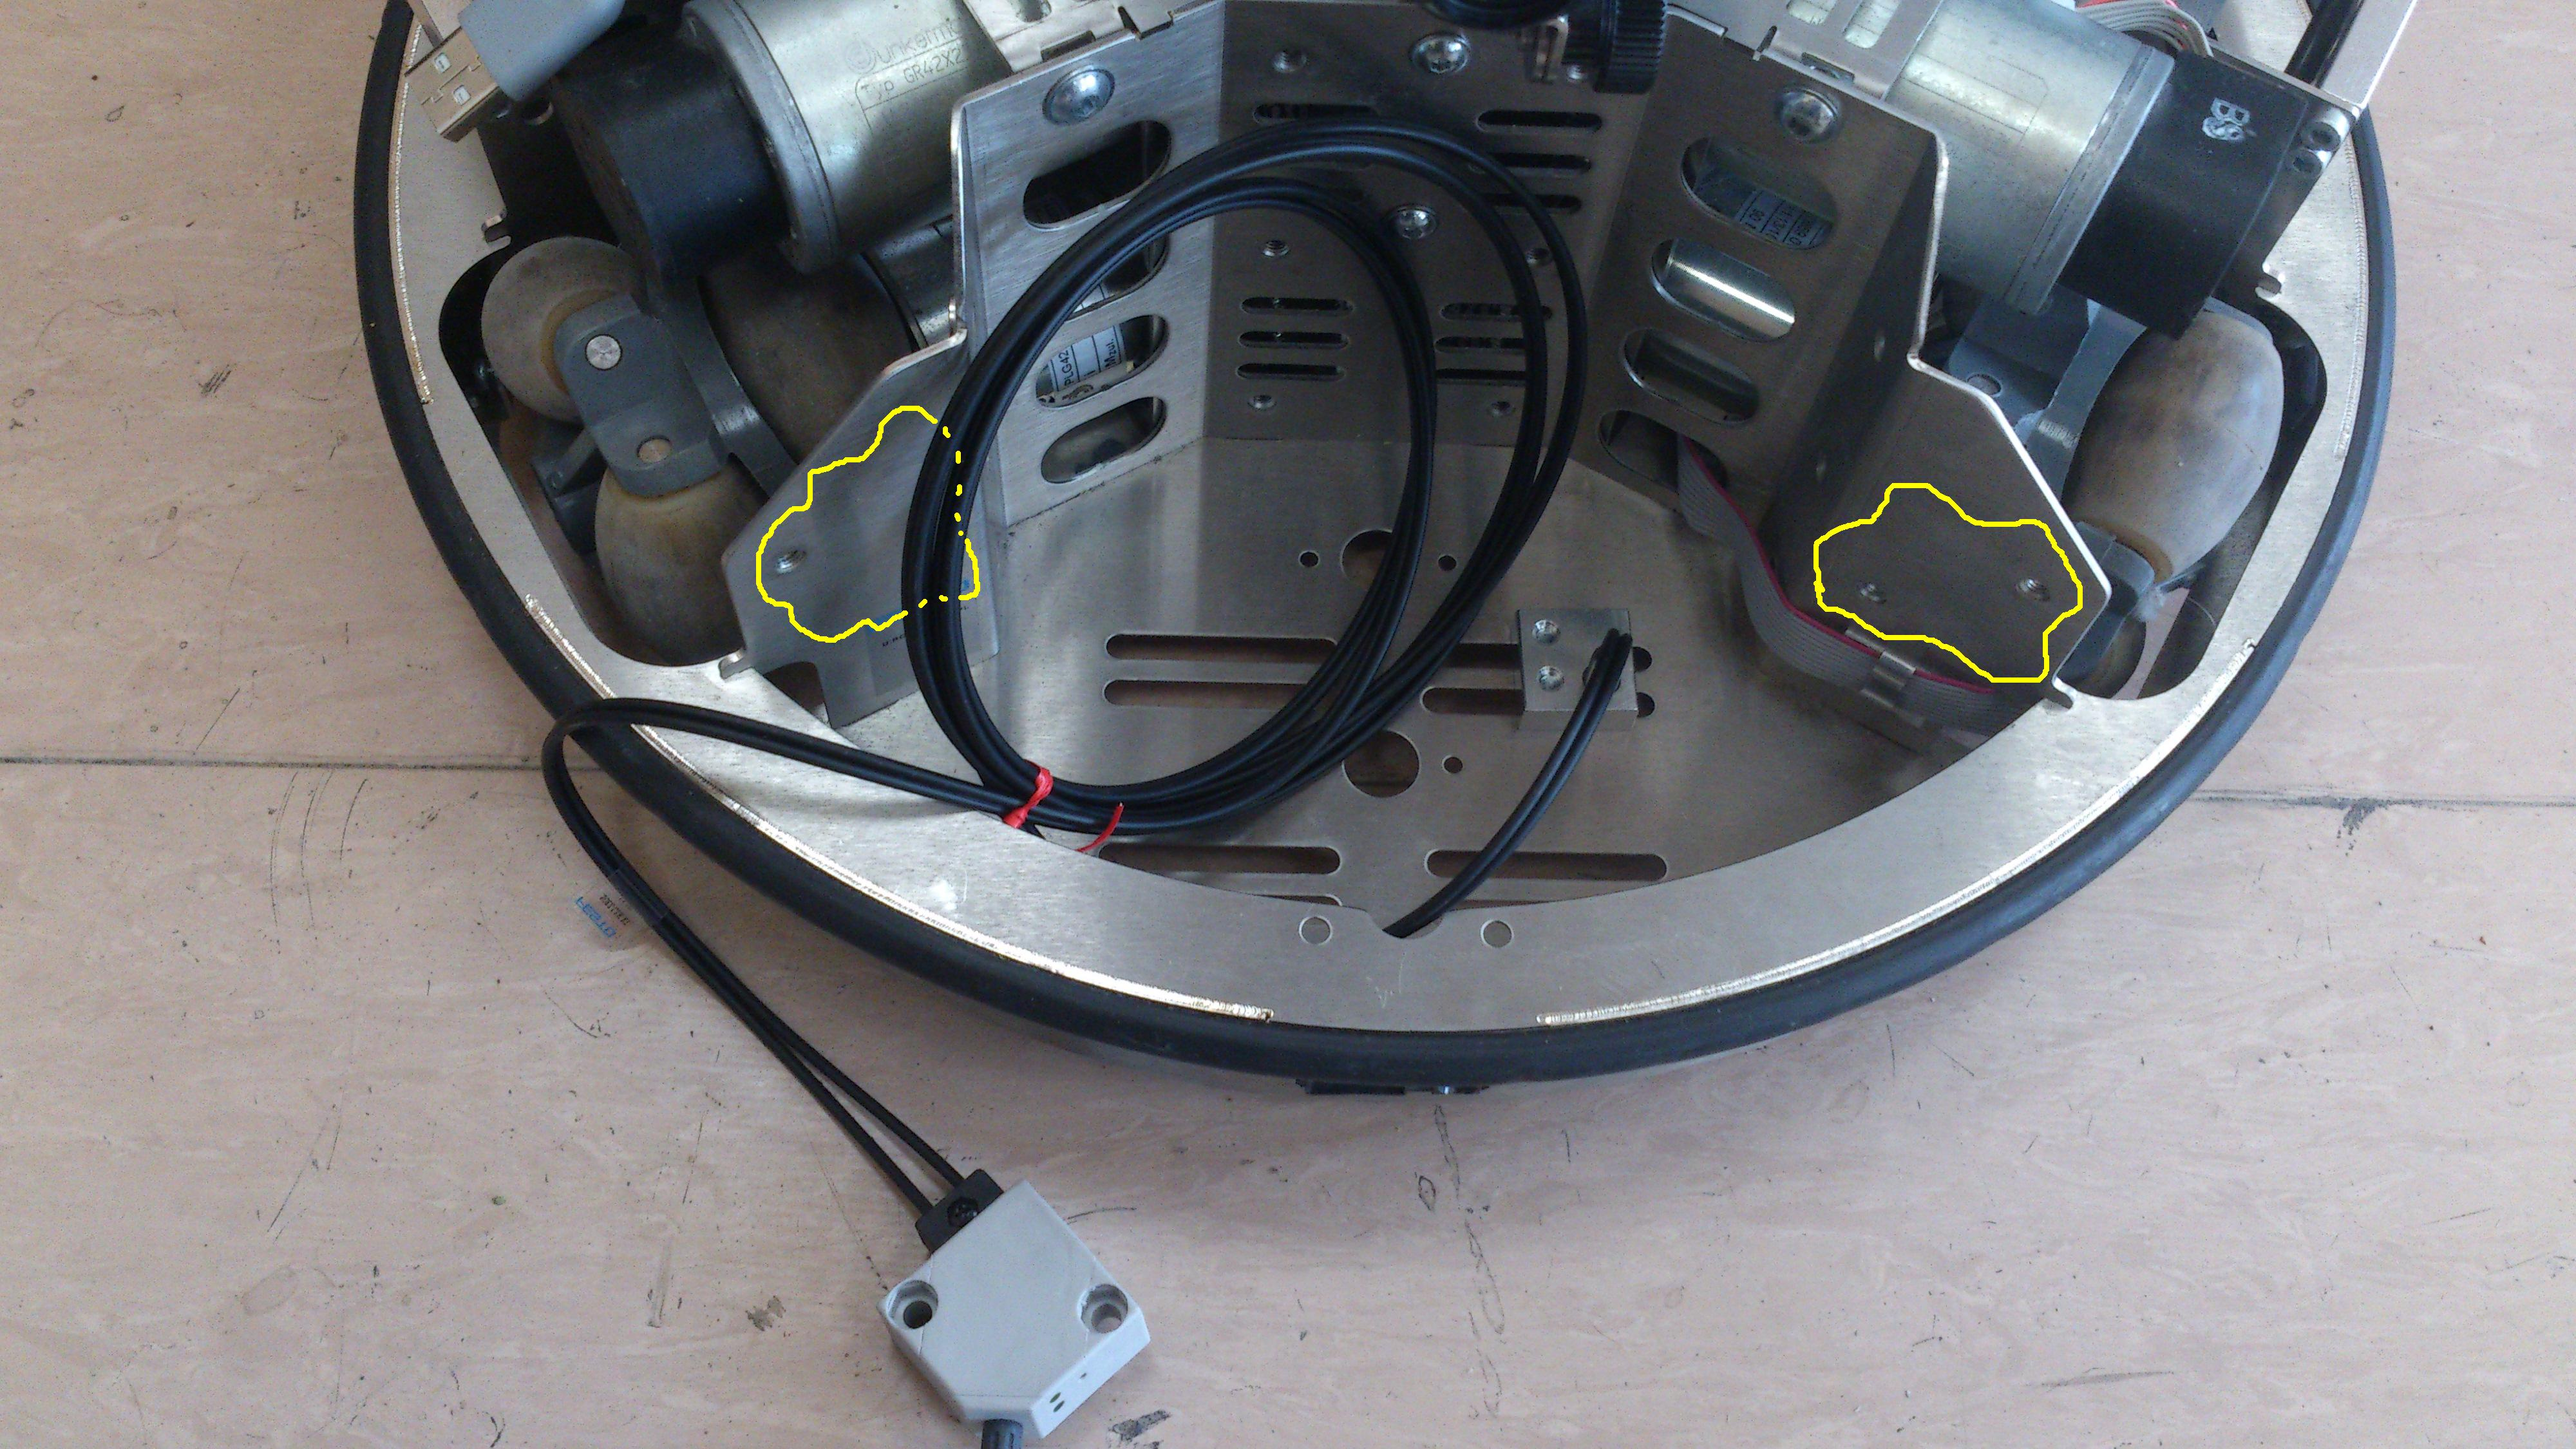
\includegraphics[width=0.65\textwidth]{optical_connect.jpg}
	\caption{Места для крепления оптических датчиков на роботе.}
	\label{img_optical_connect}
\end{figure}

К~оптическим датчикам дополнительно можно подключать световоды.
Они бывают сдвоенными и одиночными.
Сдвоенные следует применять, когда эти сенсоры применяются для определения цвета той или иной поверхности, одиночные~--- когда сенсоры используются как световые барьеры.
Пример использования одиночных световодов доступен в подразделе~\ref{part_gripper_connect}, а сдвоенного~--- на рисунке~\ref{img_optical_connect}.
На нем показан способ установки светочувствительного конца такого световода на днище робота, к которому можно прибегнуть, когда необходимо наделить робота умением определять цвет дорожного полотна.

Для установки световодов просто воткните их свободные концы в отверстия излучателя и приемника (см.~рисунок~\ref{img_optical}) и закрепите их там некоторым поворотом затяжного винта.

Необходимо отметить, что даже при правильном выполнении всех выше описанных действий датчики могут <<не заработать>>.
Это можно исправить, покрутив маленькой отверткой настроечный винт, которым регулируется дальность срабатывания сенсоров (см.~рисунок~\ref{img_setting_screw}).

\begin{figure}[h!]
	\centering
	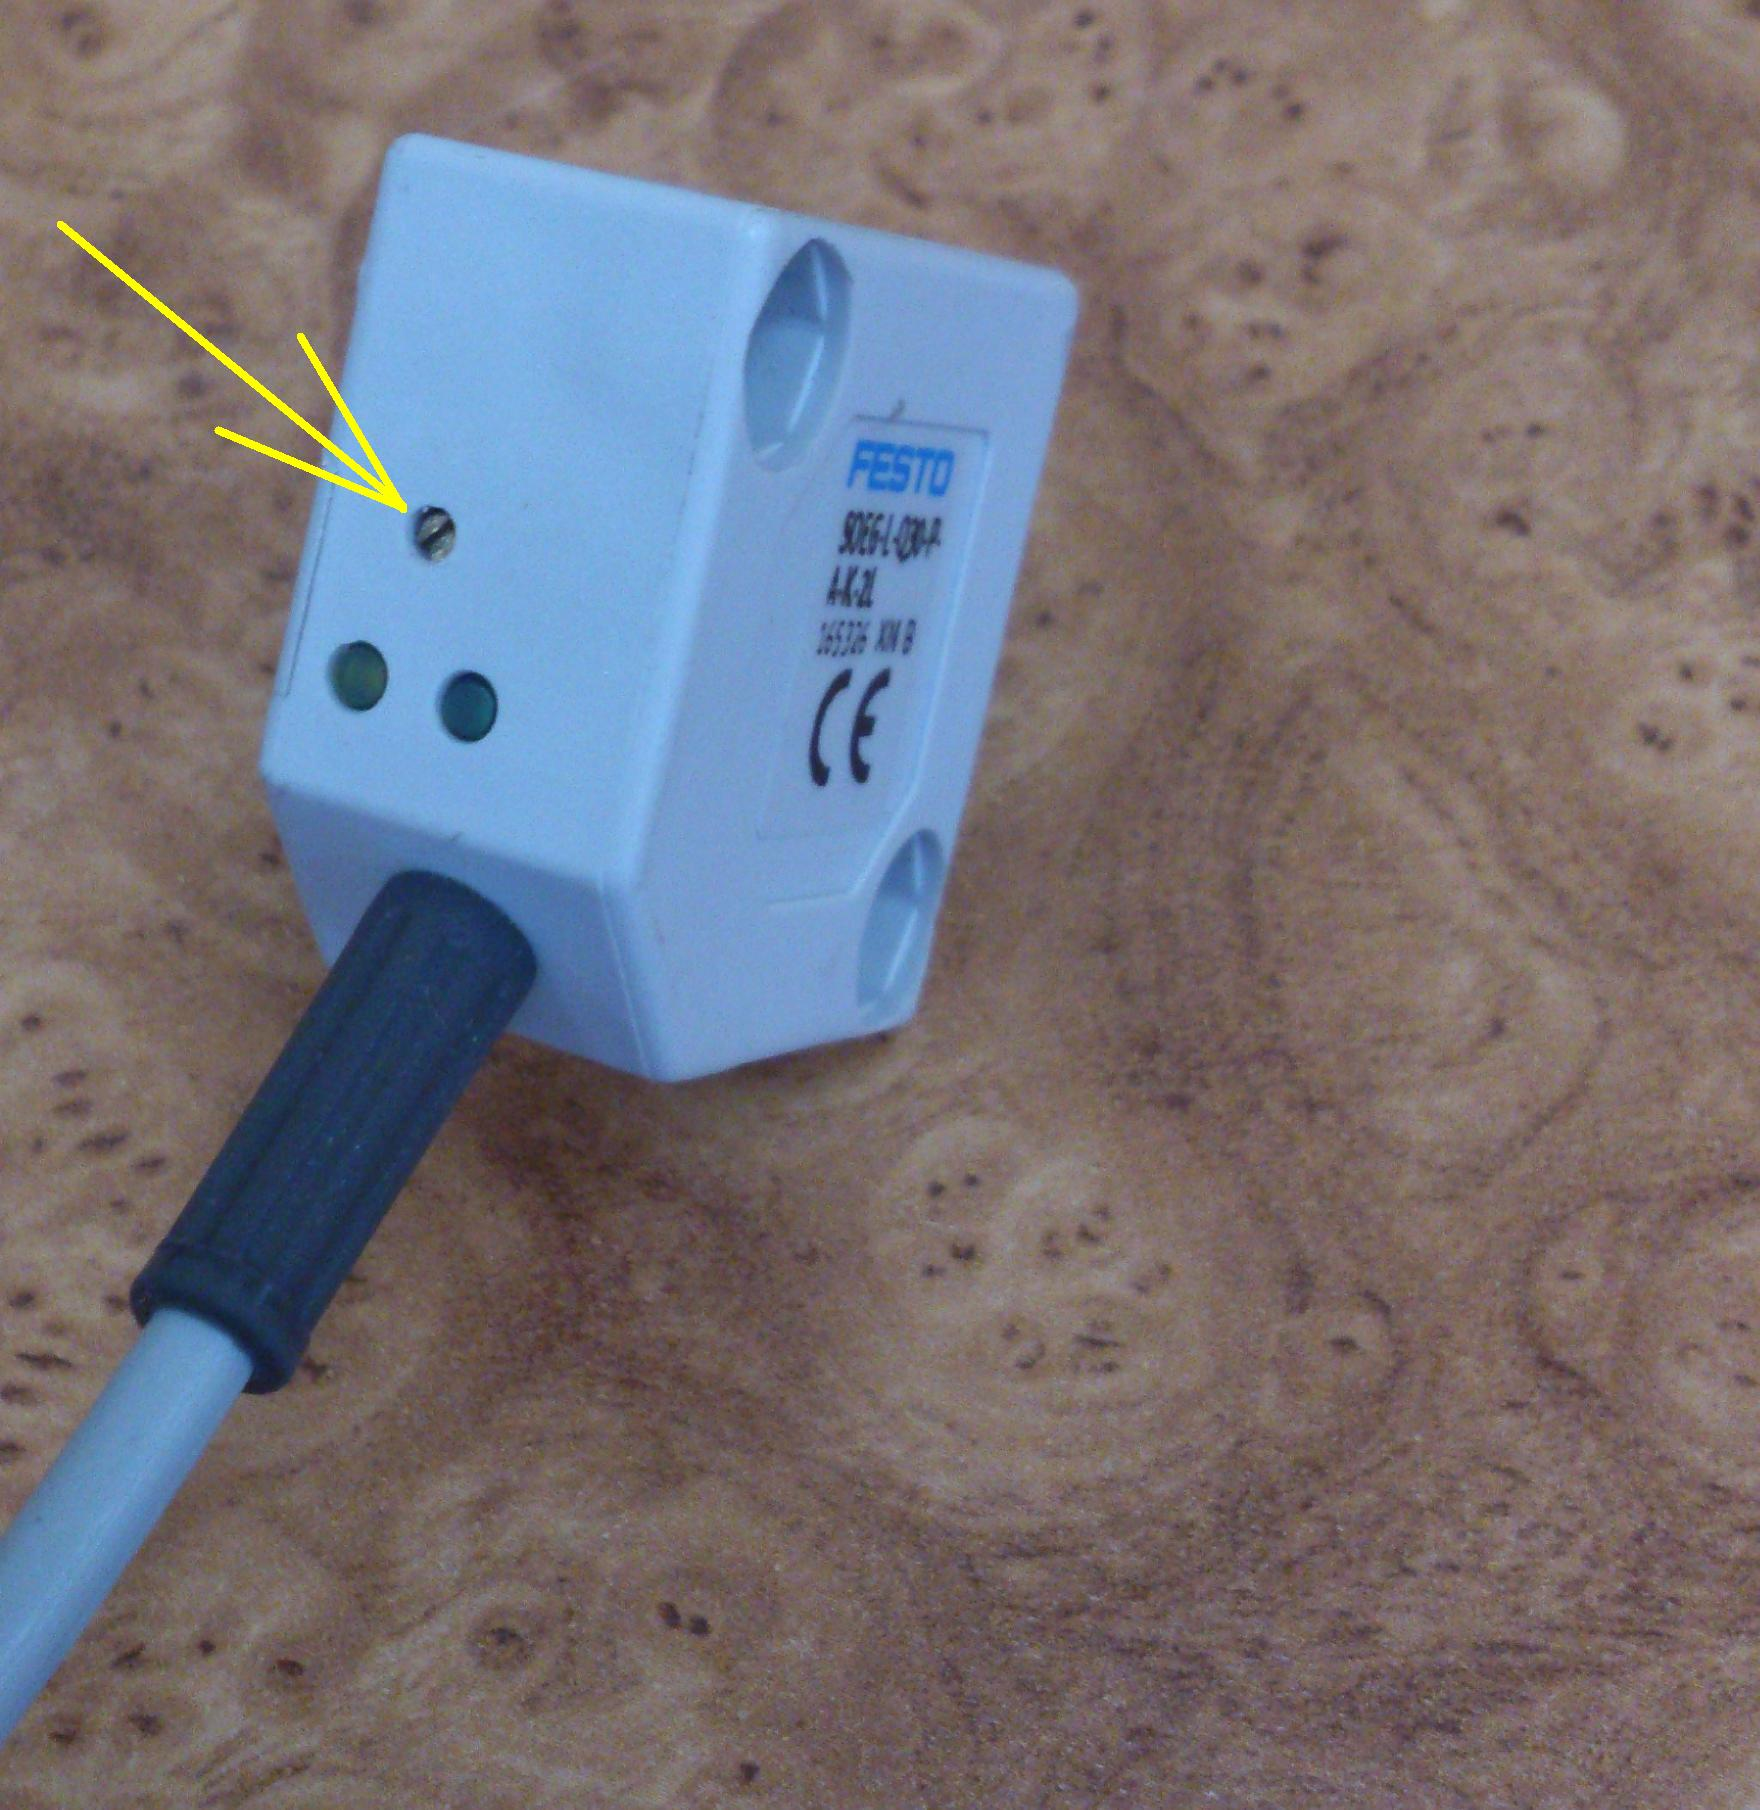
\includegraphics[width=0.35\textwidth]{setting_screw.jpg}
	\caption{Местоположение на оптическом сенсоре регулировочного винта.}
	\label{img_setting_screw}
\end{figure}



\subsection{Подключение схвата (gripper)}\label{part_gripper_connect}
Доступный для подключения к Robotino схват раскрывается всего на 4--4.5~мм (см.~рисунок~\ref{img_gripper_op_cl}): расстояние между внутренними поверхностями его пальцев в закрытом состоянии составляет~$38.5$~мм, в открытом~---~$43$~мм.

\begin{figure}[h]
	\begin{minipage}[h]{0.49\linewidth}
		\centering{ 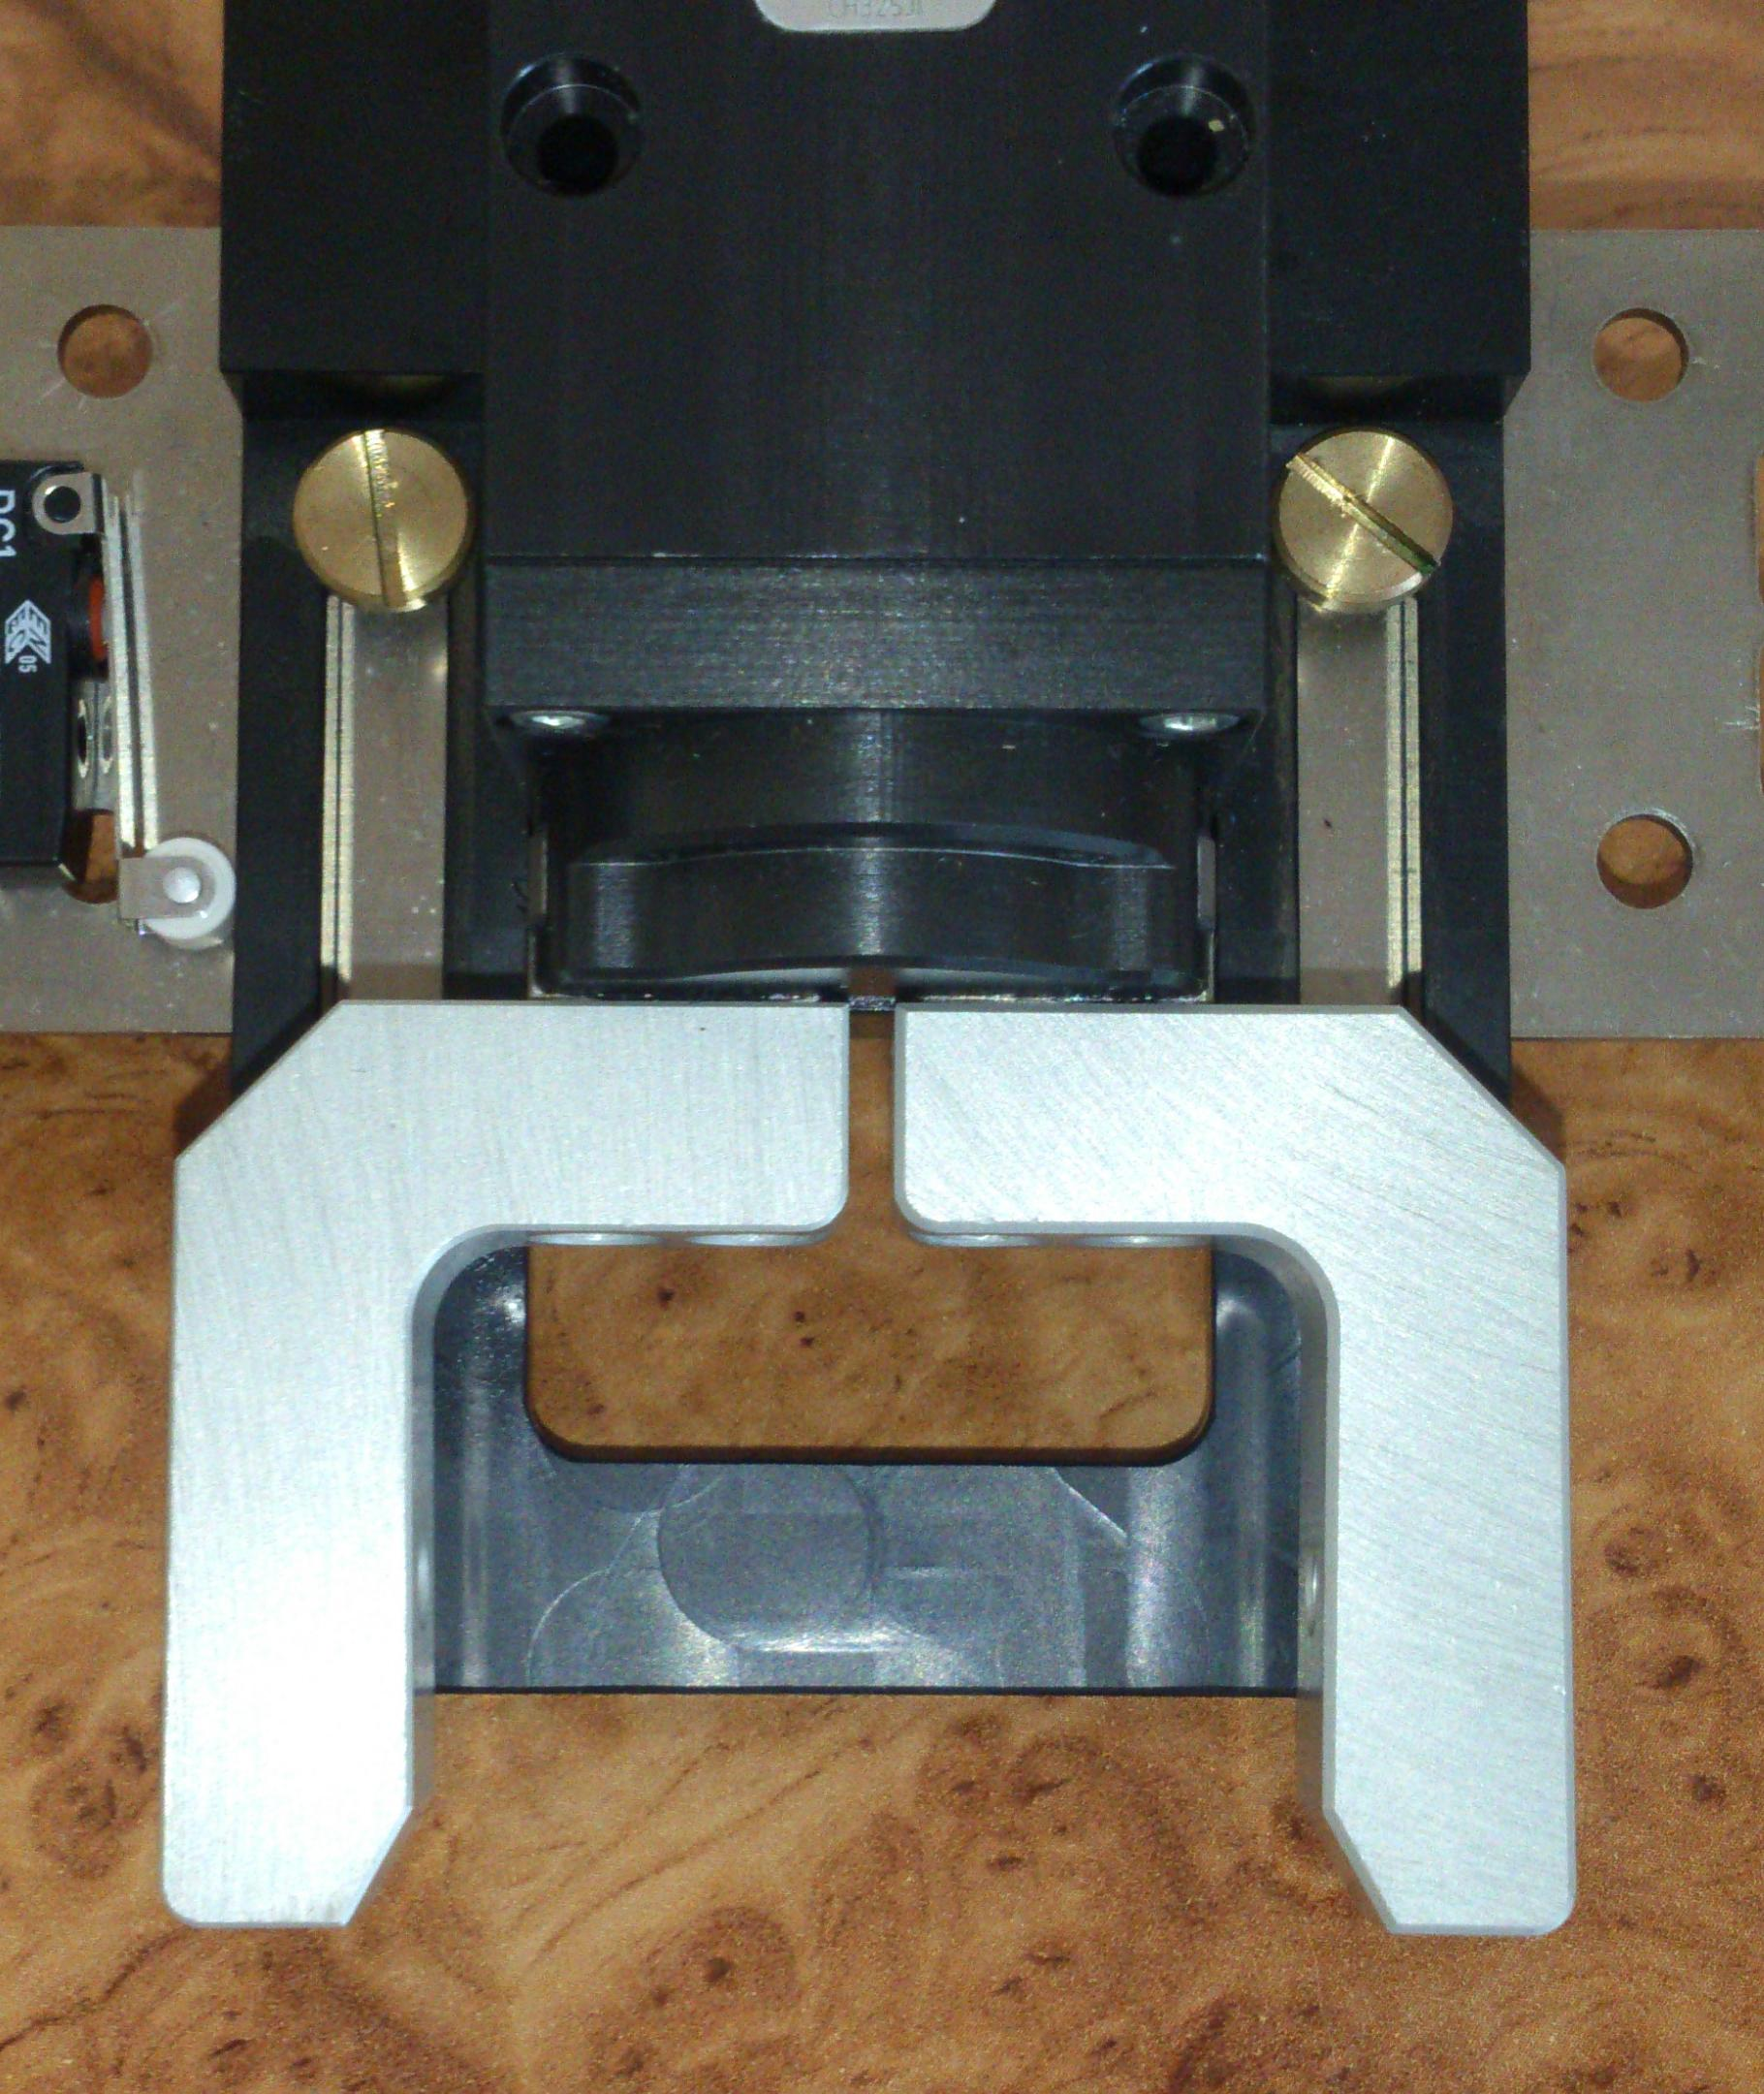
\includegraphics[height = 6cm]{gripper_closed.jpg} }
	\end{minipage}
	\hfill
	\begin{minipage}[h]{0.49\linewidth}
		\centering{ 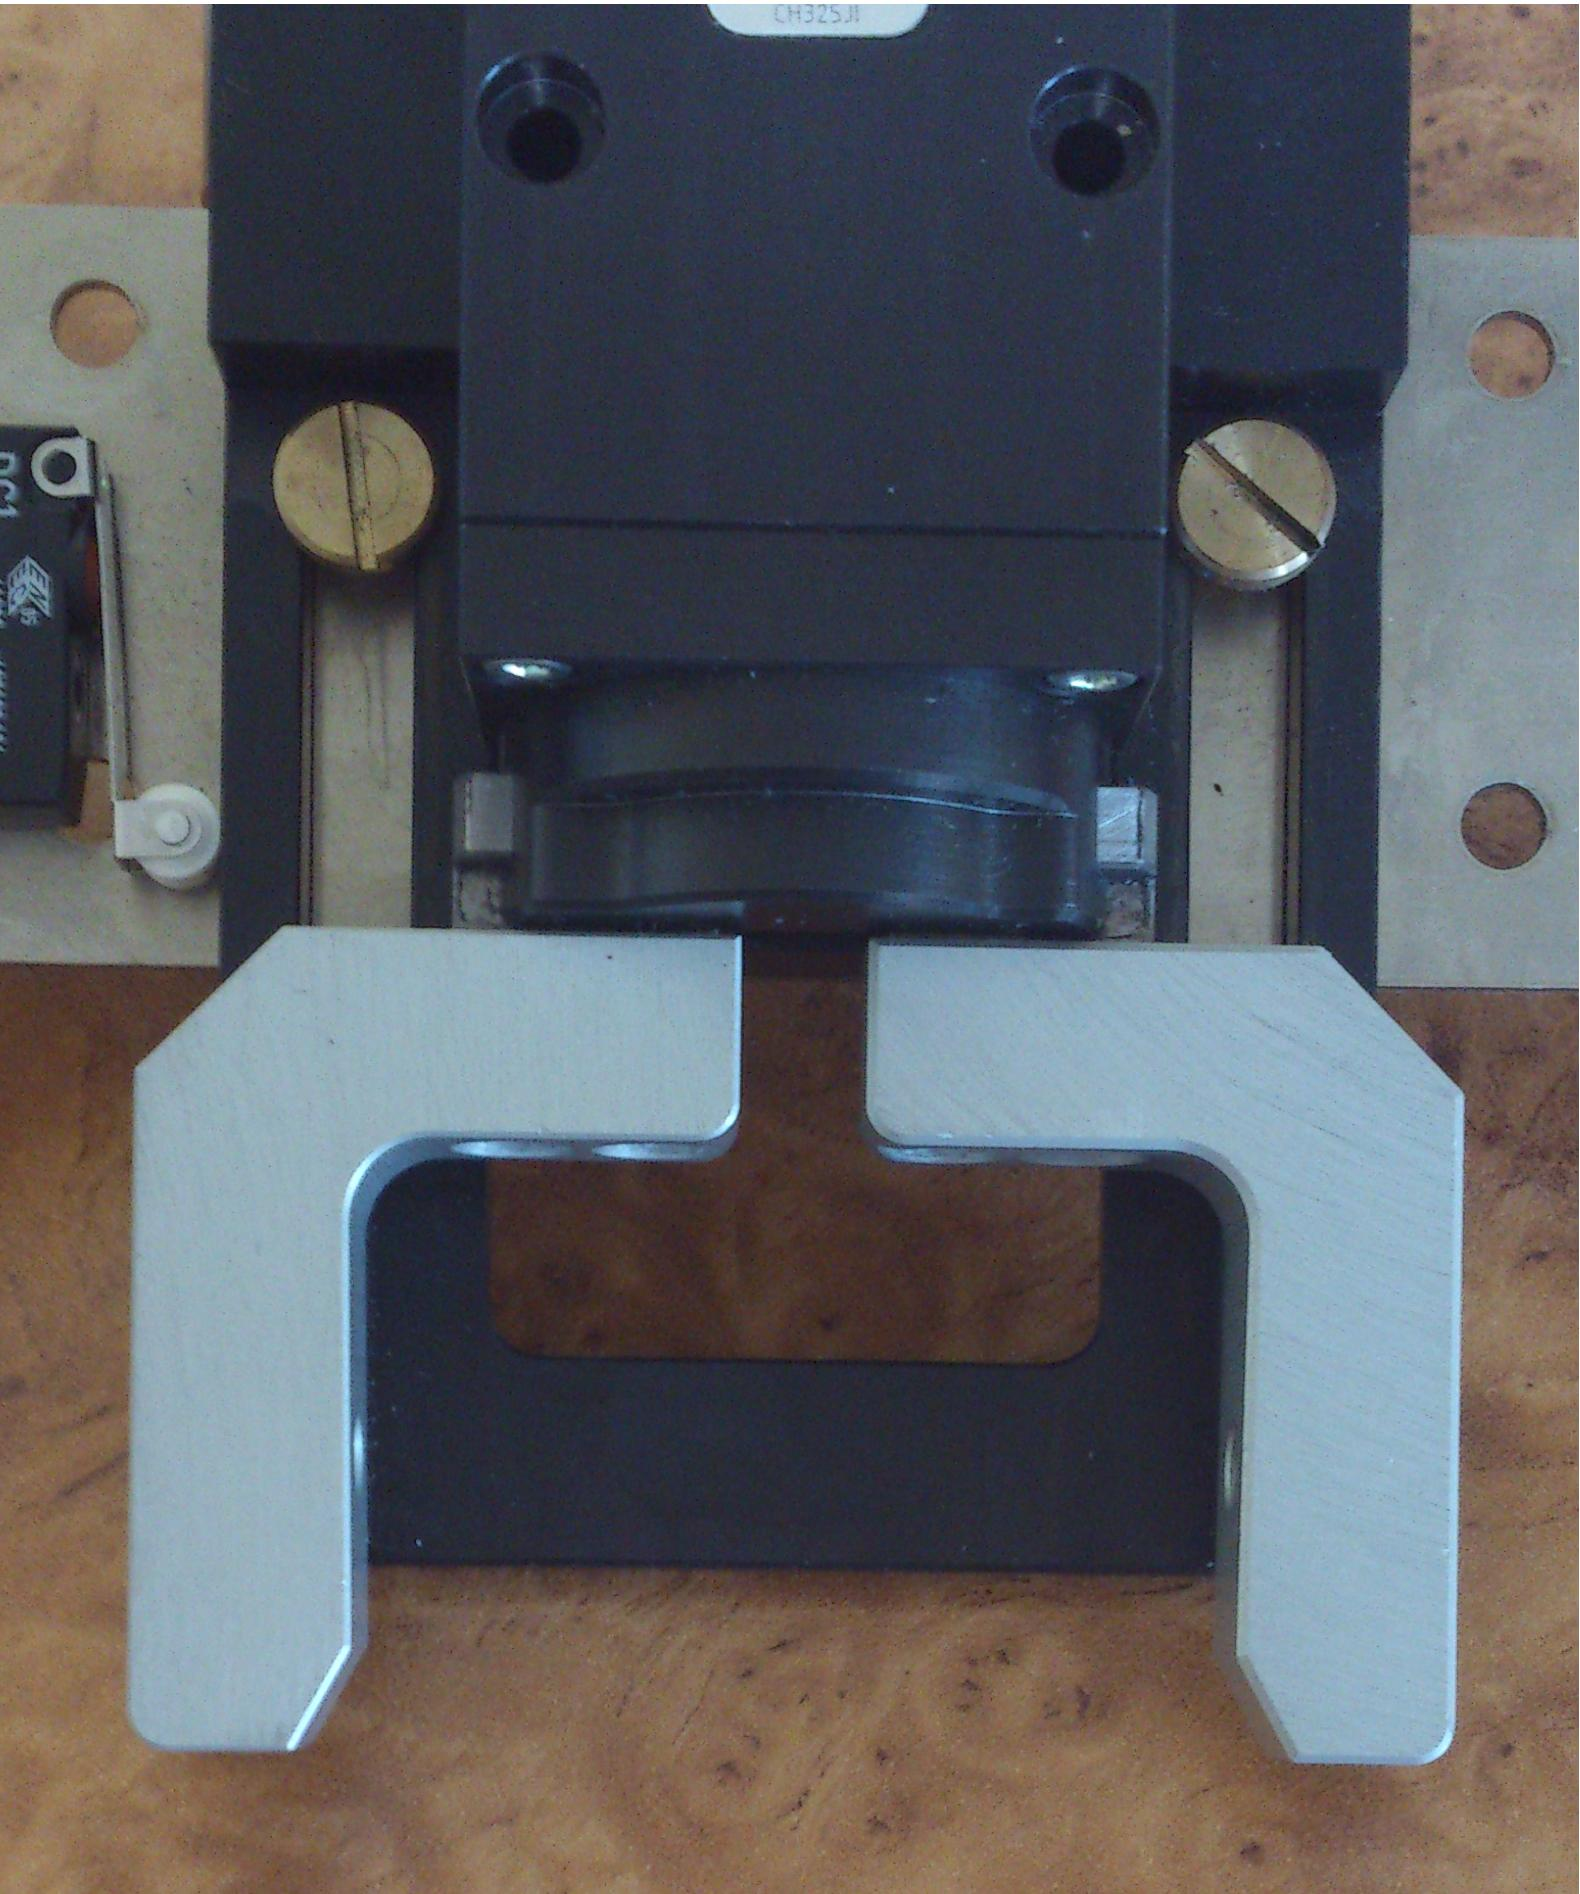
\includegraphics[height = 6cm]{gripper_opened.jpg} }
	\end{minipage}
	\caption{Схват робота в открытом и закрытом состояниях.}
	\label{img_gripper_op_cl}
\end{figure}

Для электрического подключения схвата прикрутите к нему прилагающийся кабель.
Последний внешне похож на те, которые применяются в паре с датчиками-металлоискателями, и отличается от них главным образом только тем, что содержит три провода: черный, коричневый и синий~--- а не четыре.
Затем снимите командный блок Robotino и его левый аккумулятор (как это сделать~--- см. подраздел~\ref{part_charging}).
На открывшейся вашему взору плате найдите свободный клеммник~X15 (см.~рисунок~\ref{img_x15}).
Подсоедините к его левому гнезду коричневый провод кабеля схвата, а к правому~--- синий (для этого сперва немного открутите размещенные там прижимные винты, затем вставьте в гнезда концы проводов и закрутите винты).
Черный провод схвата никуда не подключается.
Верните на место аккумулятор и командный блок робота.
После этих действий схват готов к работе.

Рекомендуемое официальным разработчиком место размещения схвата, можно посмотреть в~\cite{gripper_manual}.

\begin{figure}[h]
	\begin{minipage}[h]{0.65\linewidth}
		\centering{ 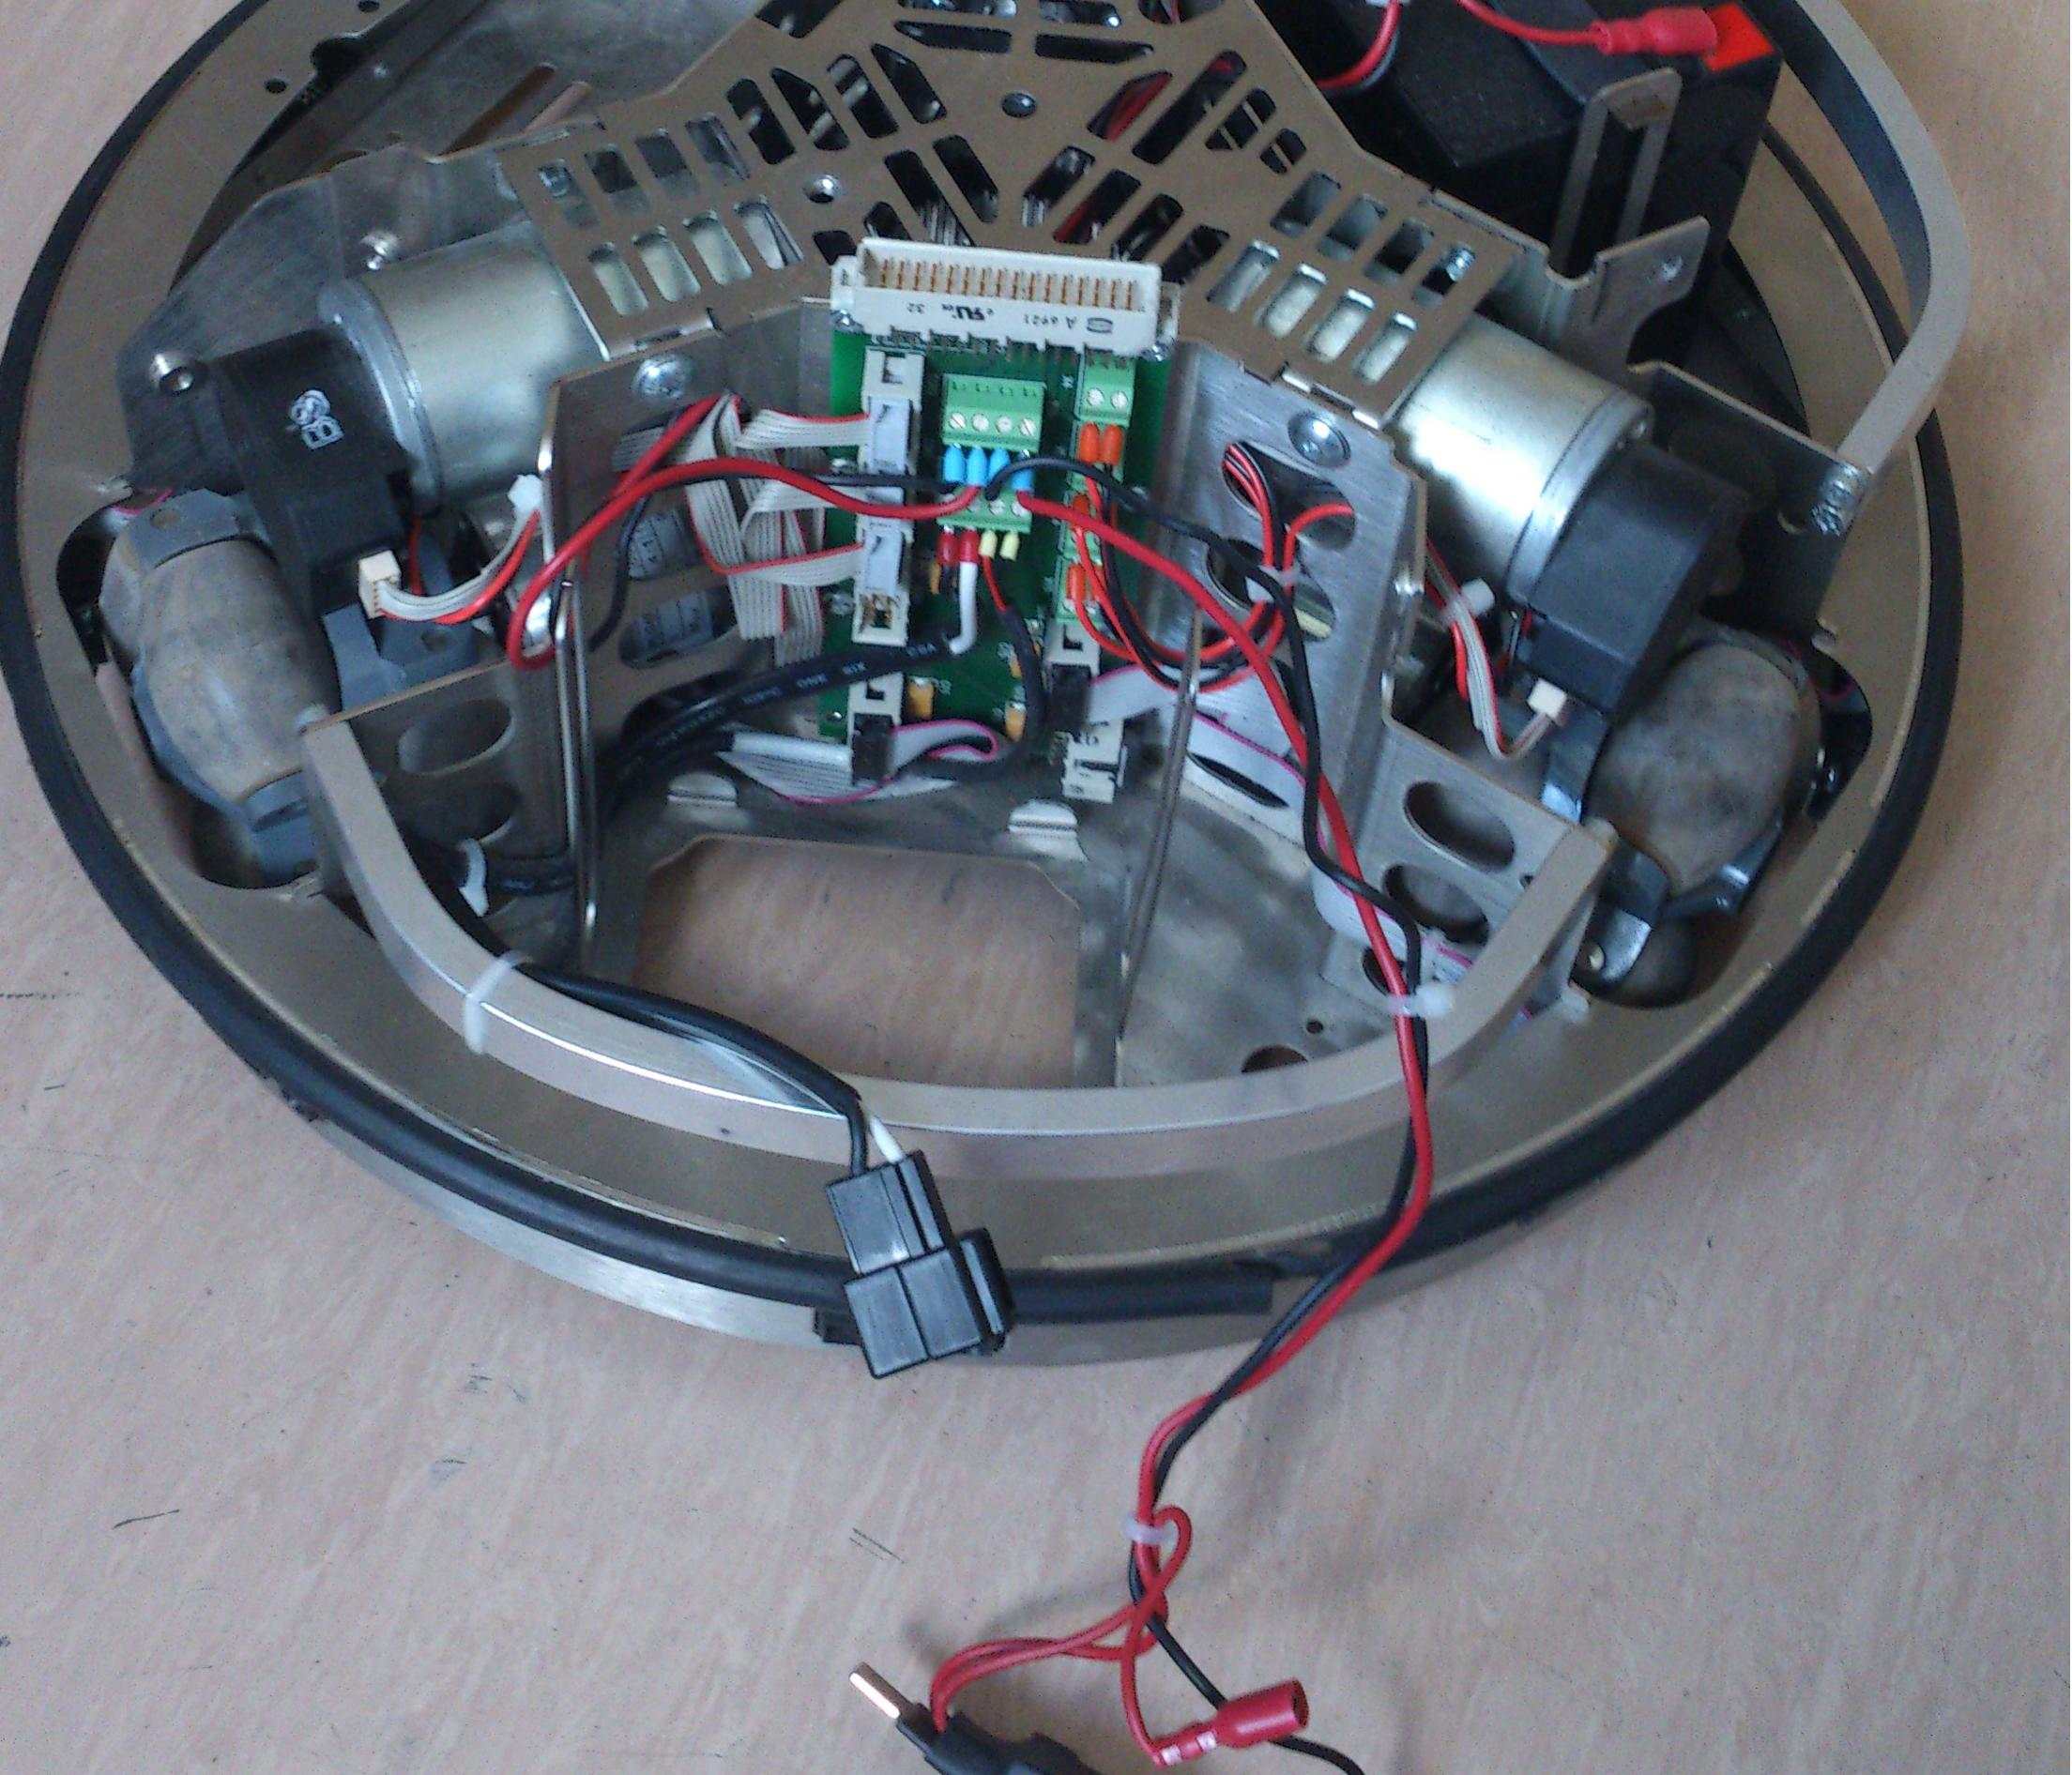
\includegraphics[height = 9cm]{x15_1.jpg} }
	\end{minipage}
	\hfill
	\begin{minipage}[h]{0.33\linewidth}
		\centering{ 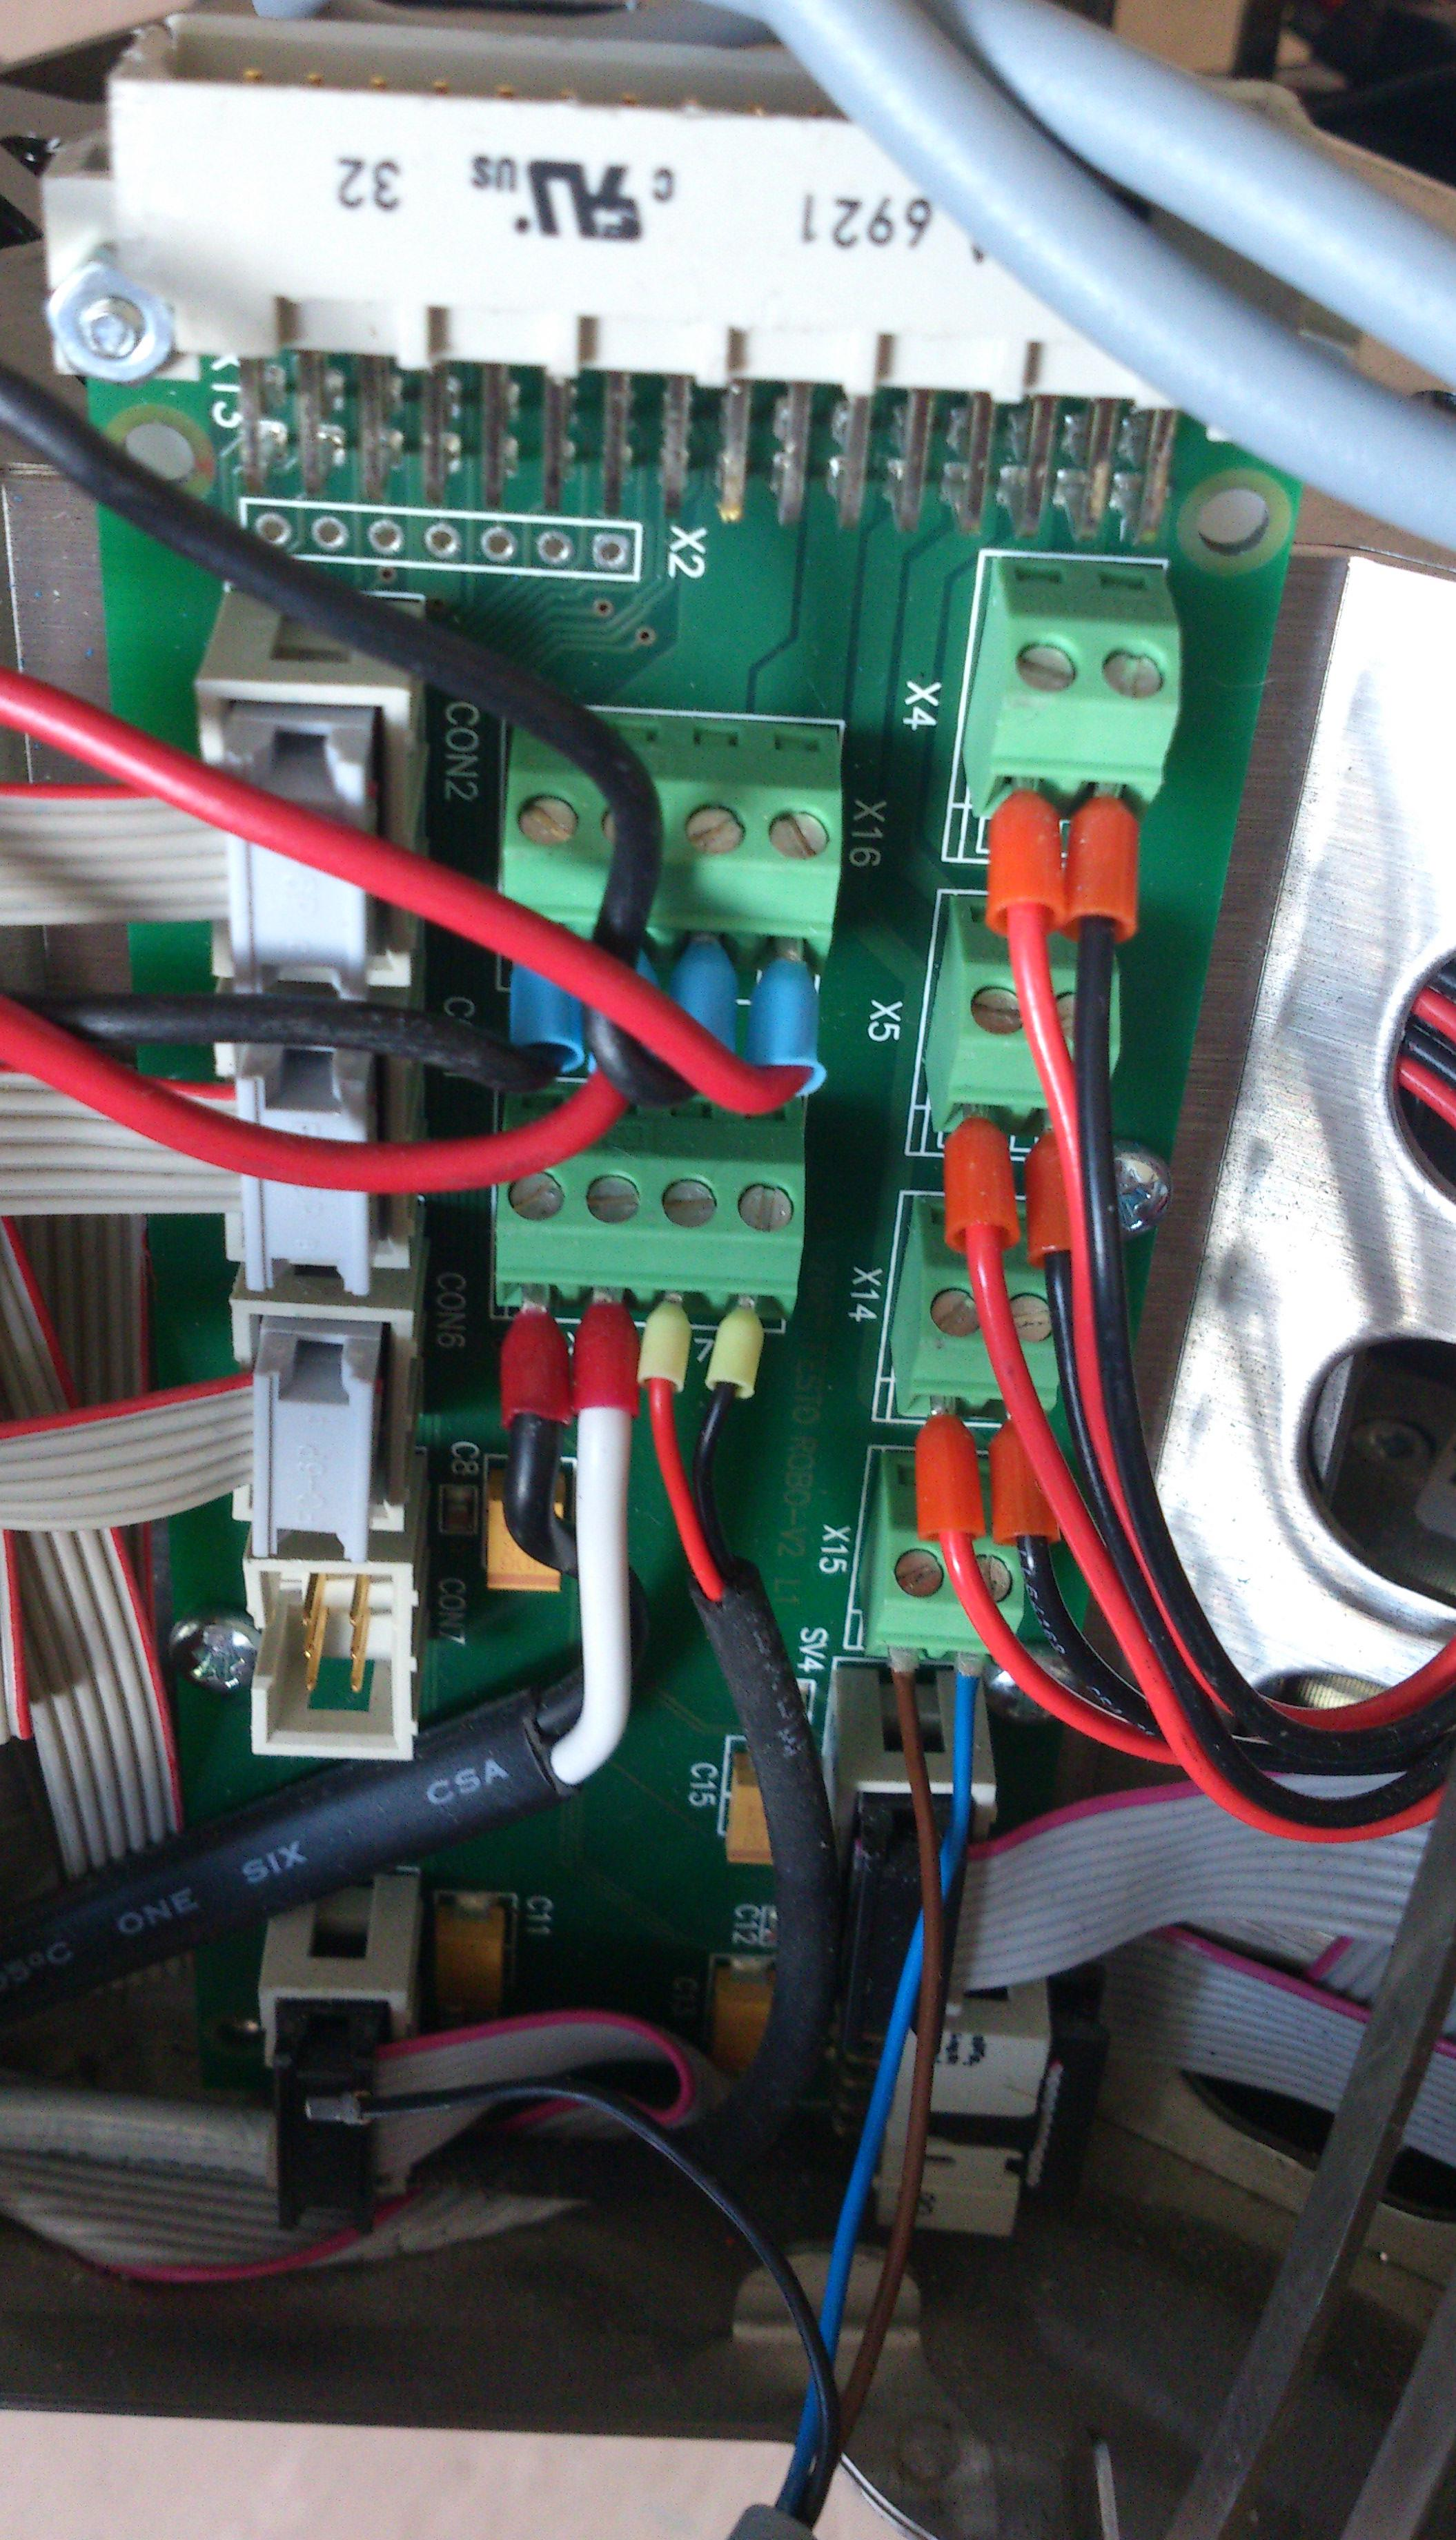
\includegraphics[height = 9cm]{x15_2.jpg} }
	\end{minipage}
	\caption{Подключение проводов к клеммнику X15.}
	\label{img_x15}
\end{figure}

На обоих пальцах схвата имеются резьбовые отверстия, в которые можно вкрутить одиночные оптоводы оптического датчика.
При этом последний, как можно догадаться, будет показывать, находится ли между пальцами схвата в данный момент что-либо или нет (см.~рисунок~\ref{img_gripper_with_barrier}).

\begin{figure}[h!]
	\centering
	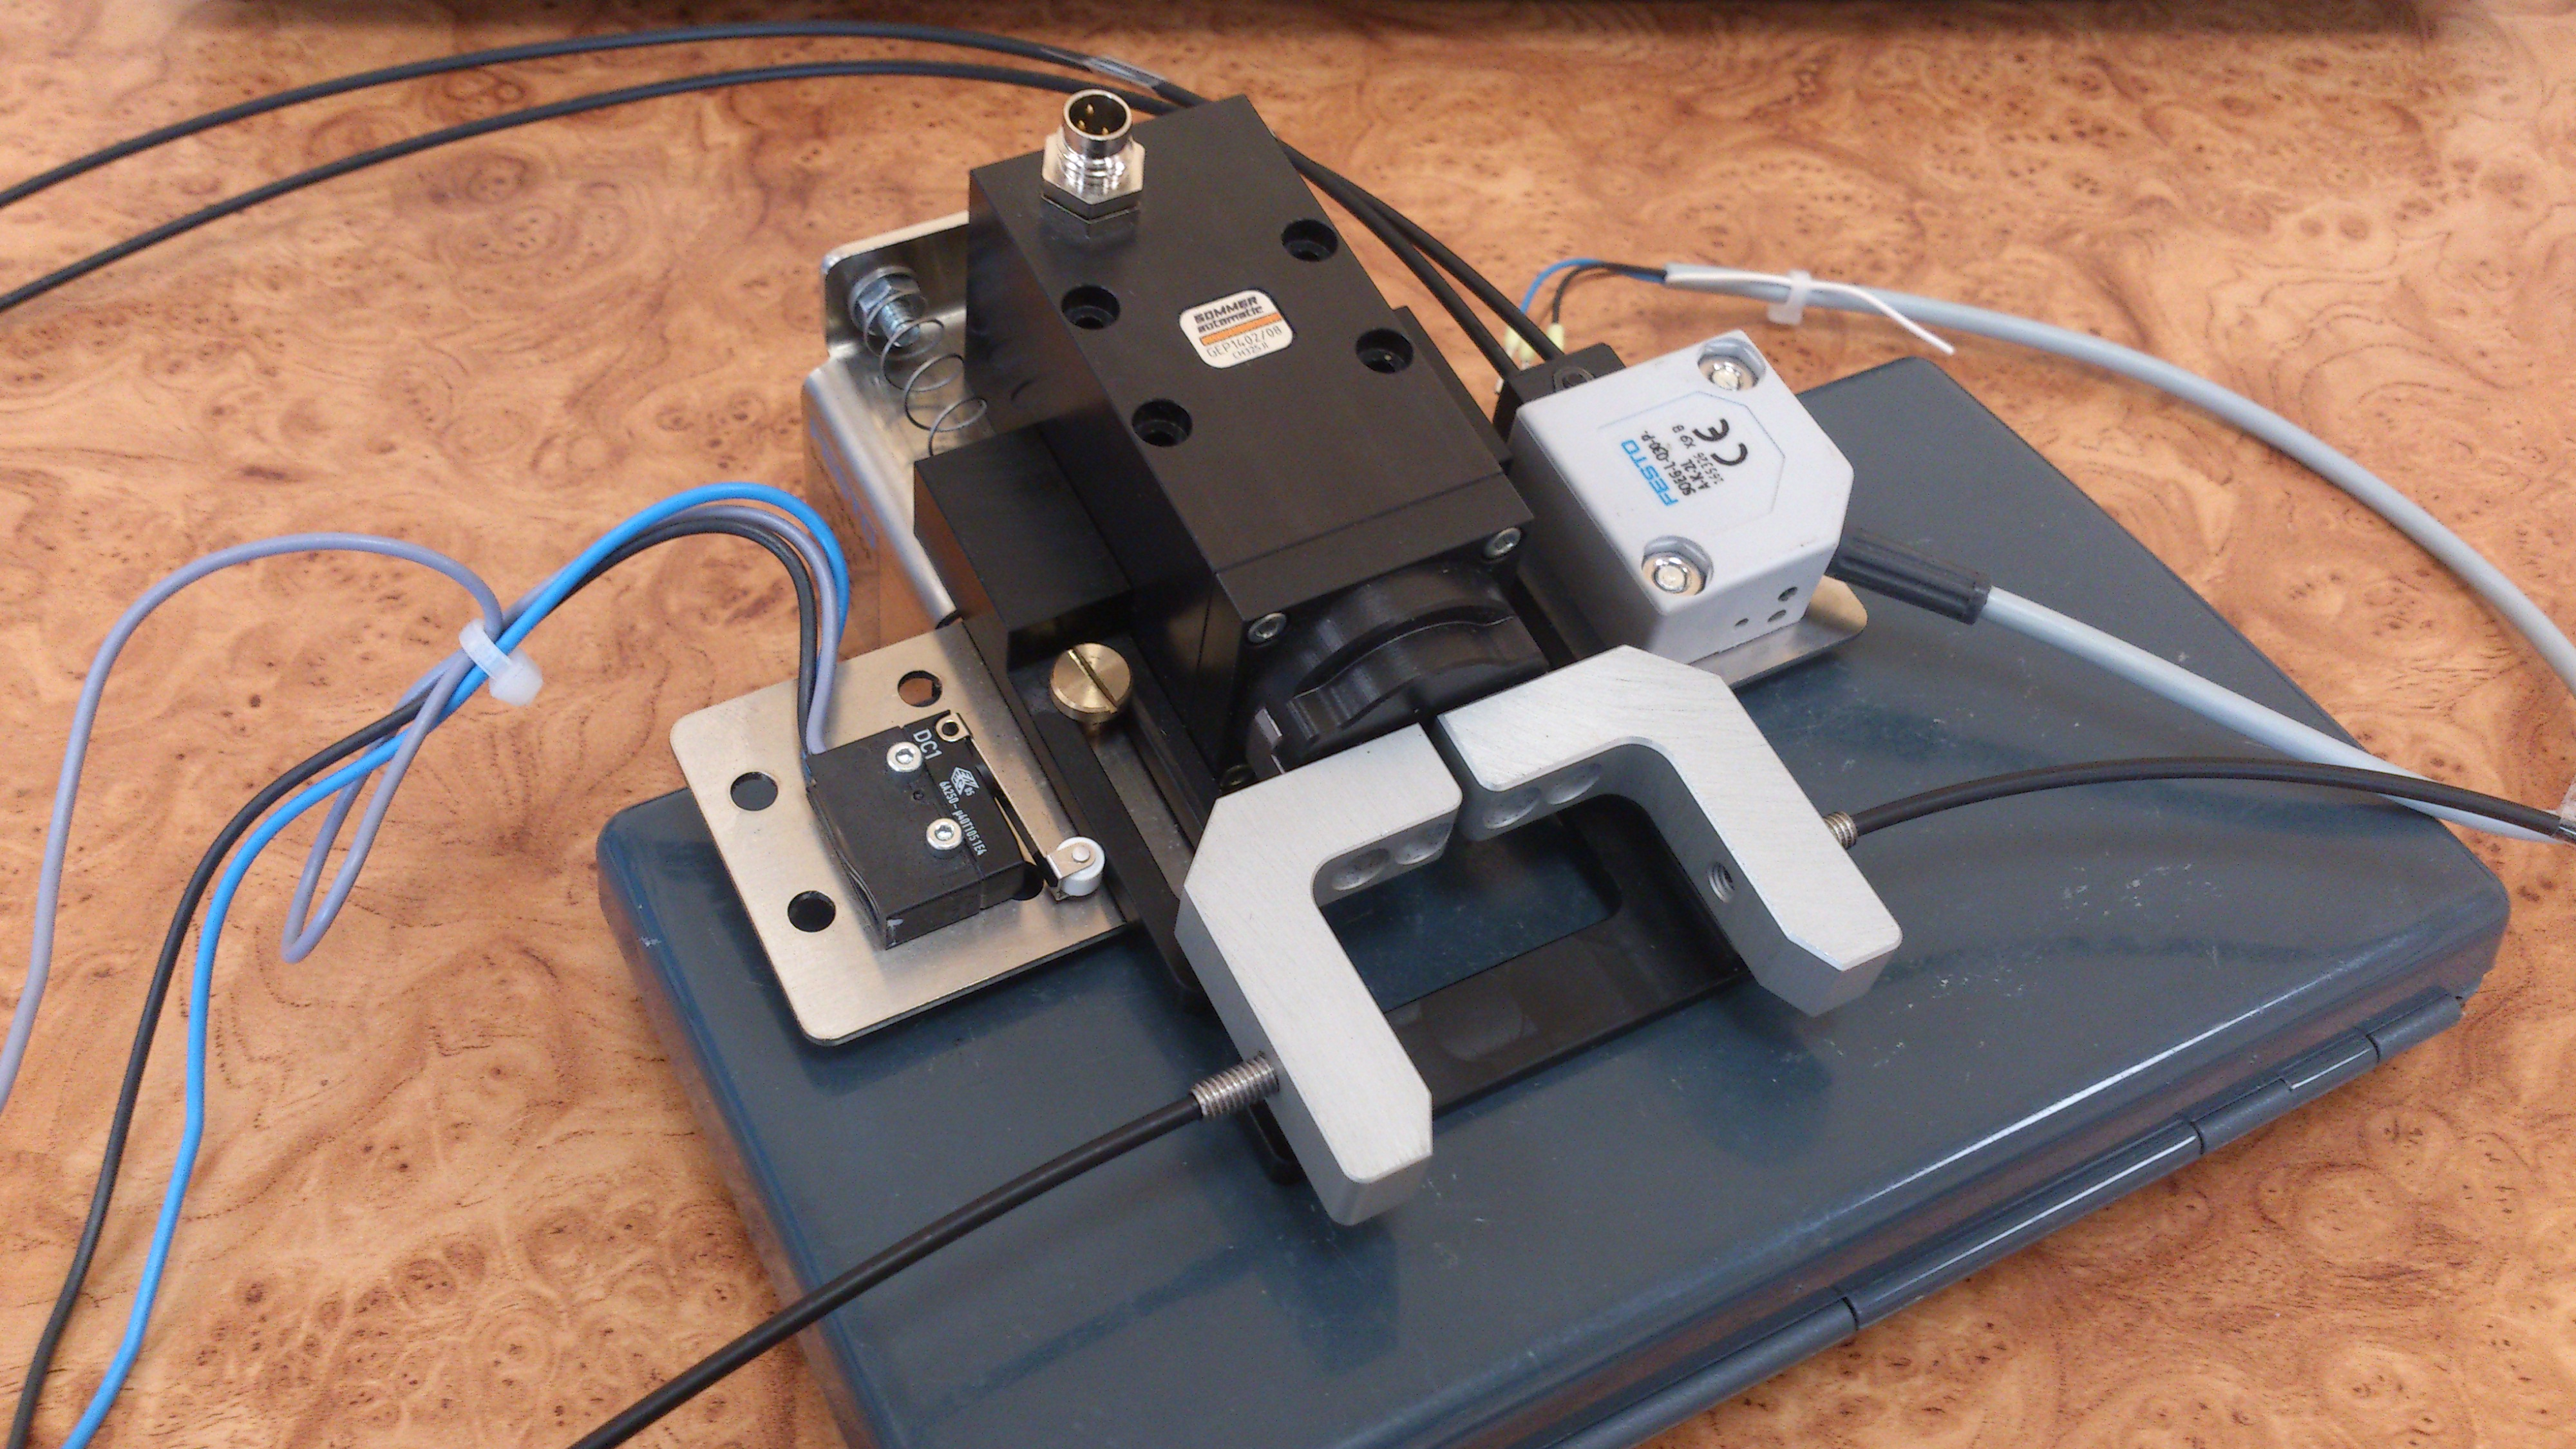
\includegraphics[width=0.8\textwidth]{gripper_with_barrier.jpg}
	\caption{Установка оптического датчика на схват.}
	\label{img_gripper_with_barrier}
\end{figure}

На кронштейн, на который монтируется захват, есть возможность установить смещающуюся пластину, пружины и реле (его подключение~--- см.~подраздел~\ref{part_relay_connect}).
Эти элементы, объединенные в такую систему, образуют датчик касания: при смещении пластины в сторону <<тела>> схвата ролик прижимной пластинки реле <<провалится>> в специально предназначенную для этого выемку в пластине, и реле изменит свое состояние (см.~рисунок~\ref{img_touch_sensor}).

\begin{figure}[h]
	\begin{minipage}[h]{0.49\linewidth}
		\center{ 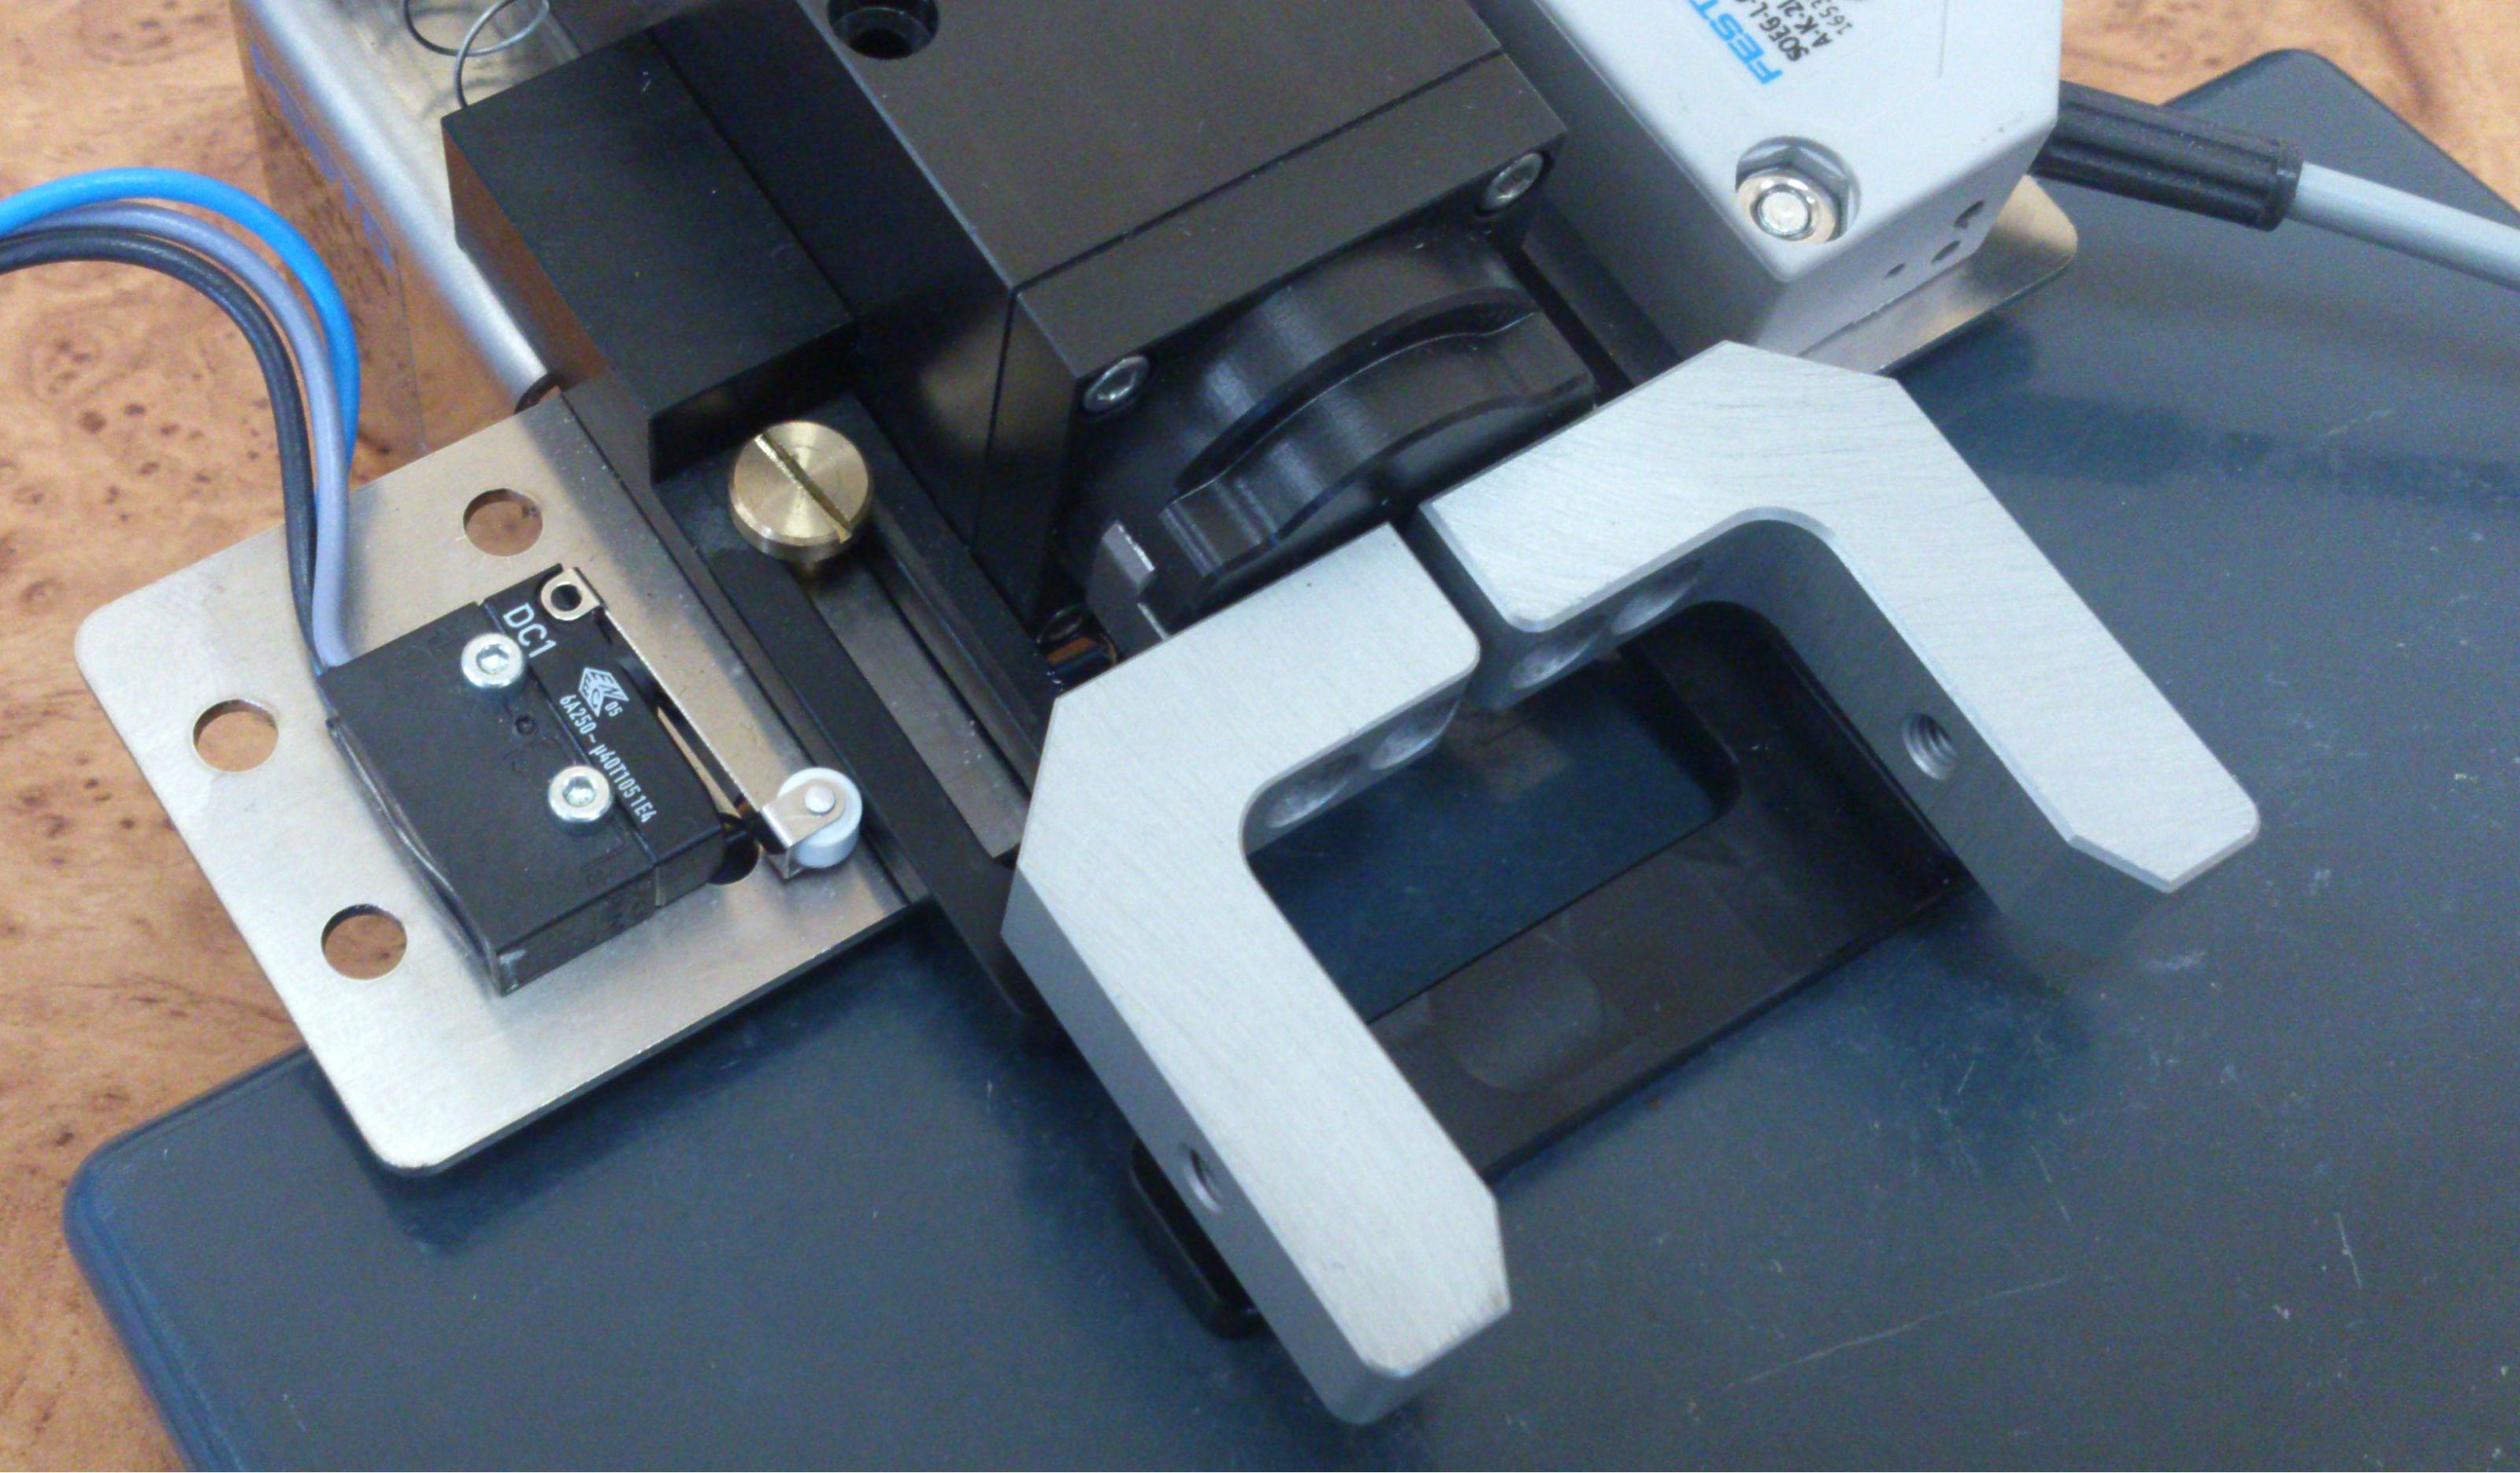
\includegraphics[height = 4.8cm]{touch_sensor_1.jpg} }
	\end{minipage}
	\hfill
	\begin{minipage}[h]{0.49\linewidth}
		\center{ 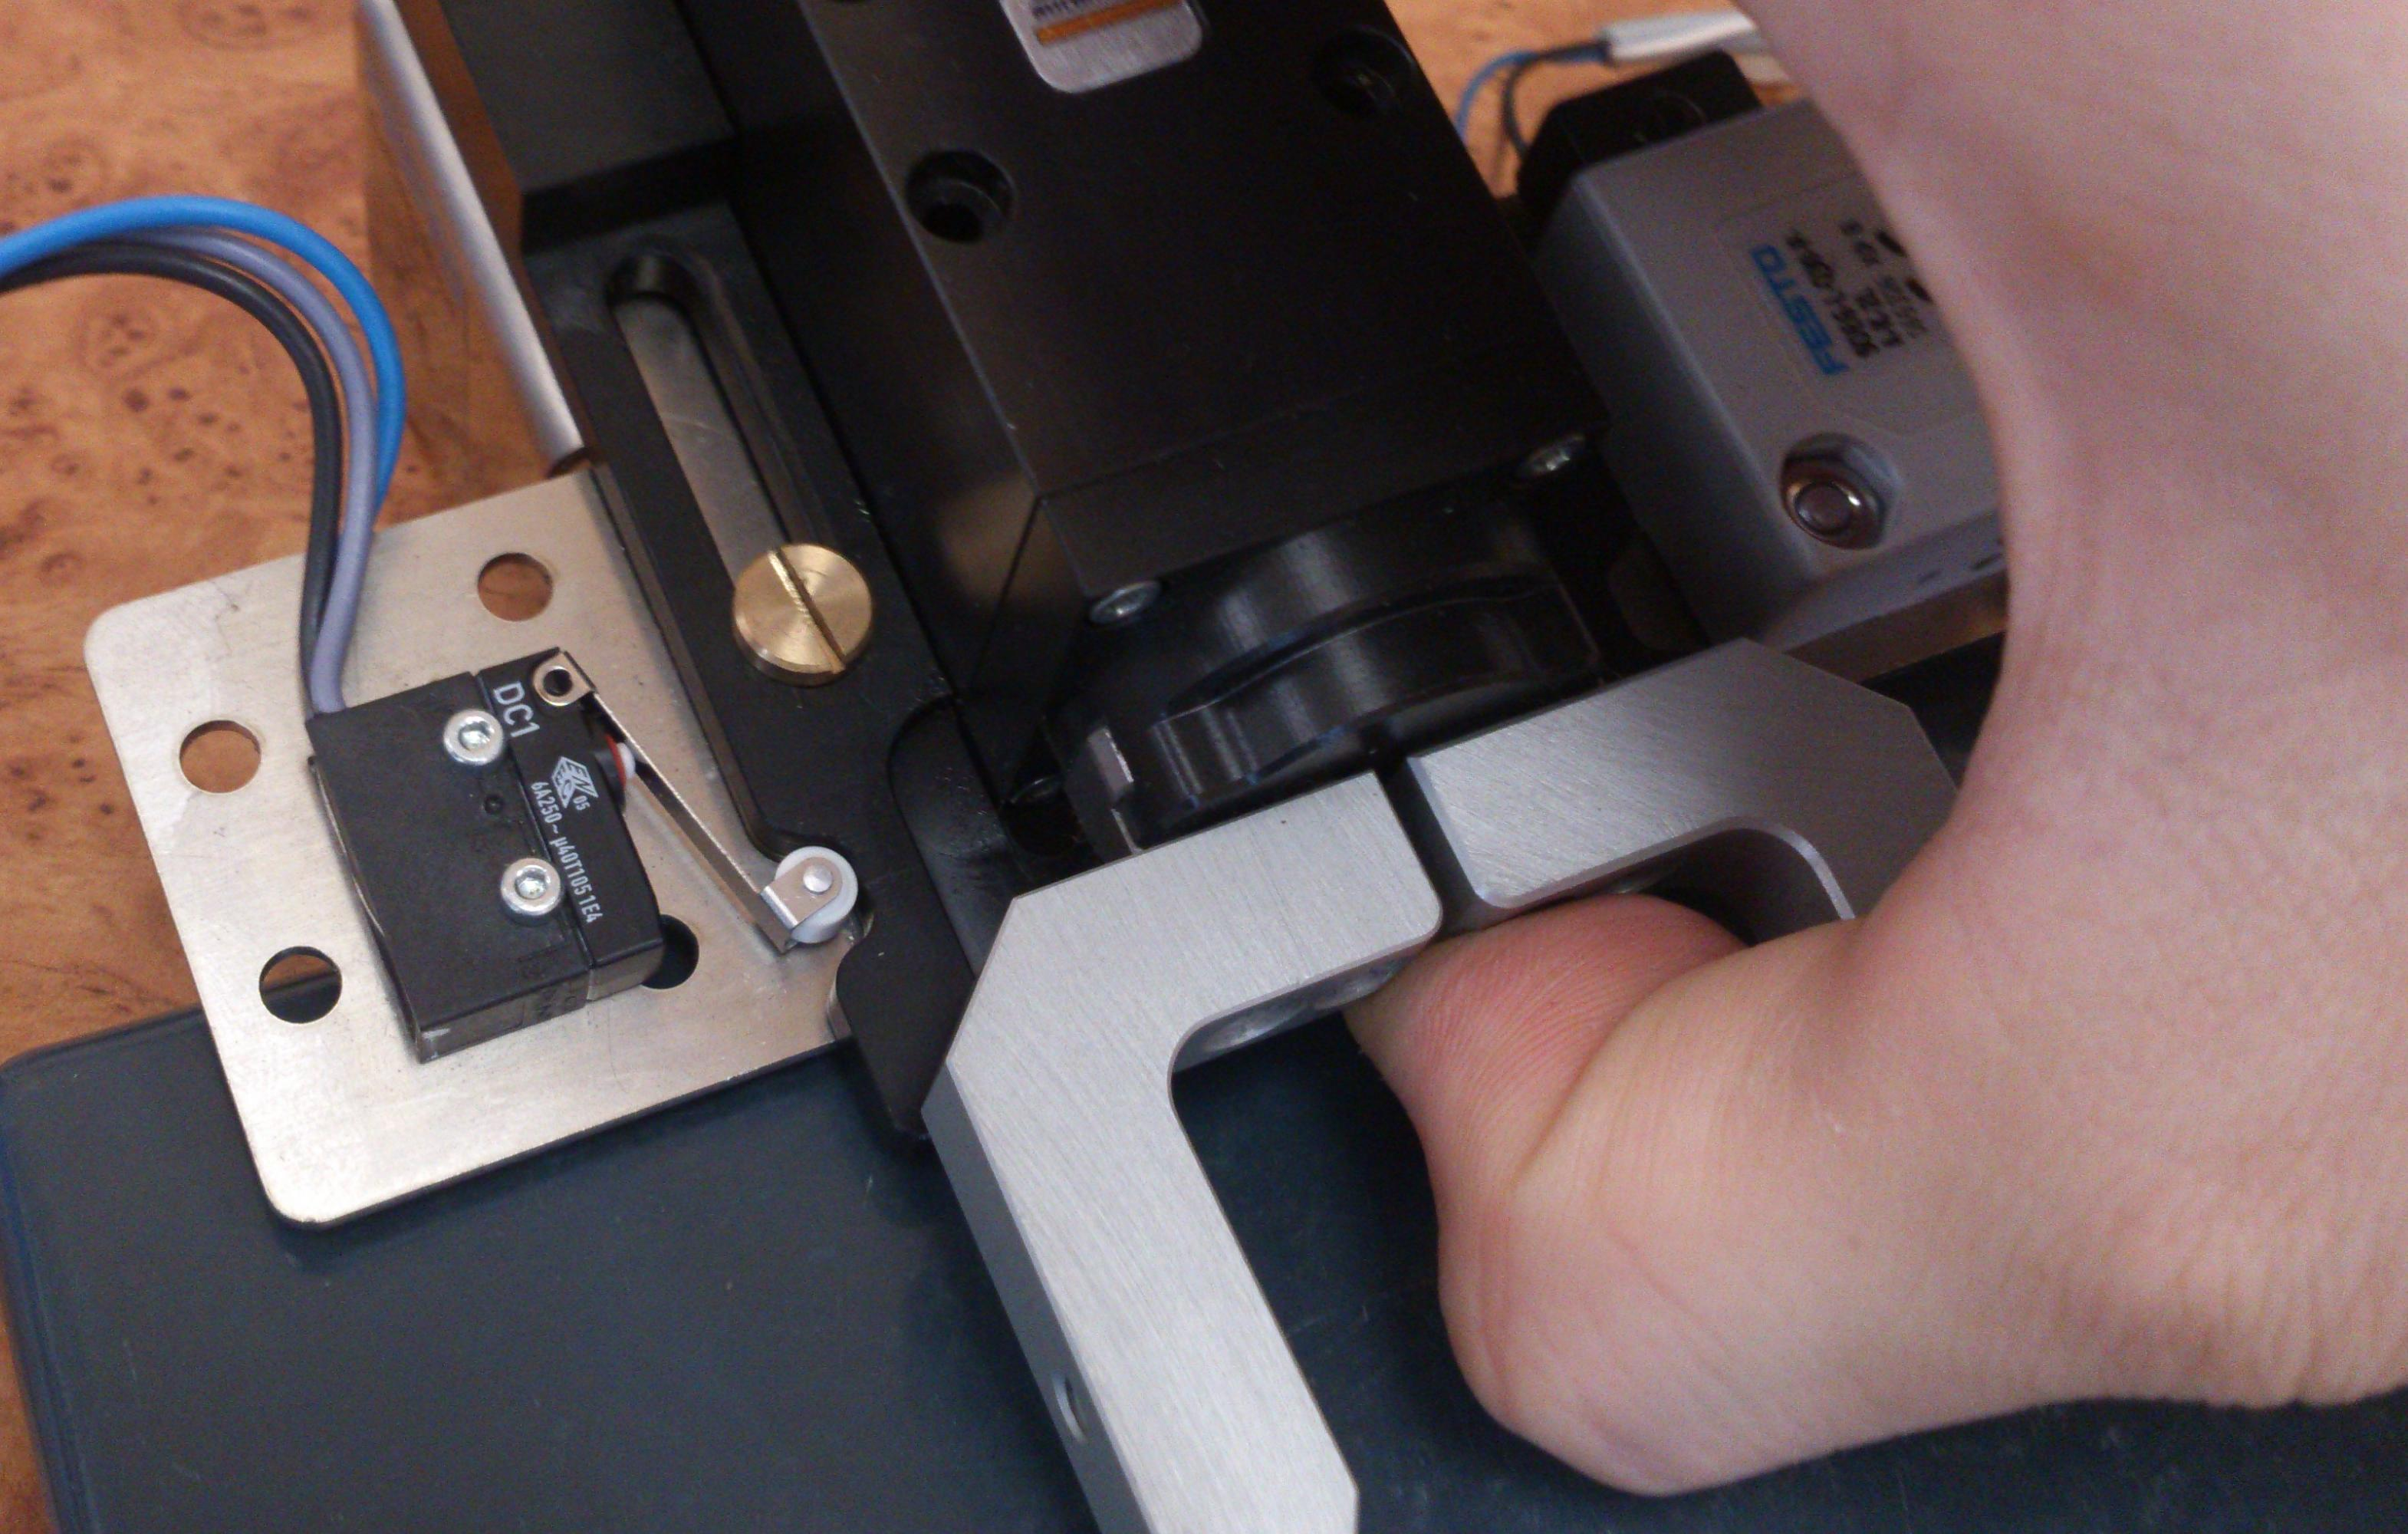
\includegraphics[height = 4.8cm]{touch_sensor_2.jpg} }
	\end{minipage}
	\caption{Принцип работы датчика касания схвата.}
	\label{img_touch_sensor}
\end{figure}



\subsection{Подключение реле}\label{part_relay_connect}
Реле, которое можно видеть на рисунках~\ref{img_gripper_with_barrier} и~\ref{img_touch_sensor}, представляет собой электромеханический переключатель с тремя проводами, способный находиться в двух состояниях.
В~первом из них (при ненажатой кнопке) он устанавливает контакт между черным и серо-голубым проводом и разъединяет между собой черный и голубой провода, во втором (при нажатой кнопке) все происходит с точностью до наоборот: появляется контакт между черным и голубым проводом, а черный и серо-голубой провода теряют соединение друг с другом.

Подключение этого реле, а в равной степени и любого другого электромеханического переключателя к роботу может быть осуществлено по схеме, изображенной на рисунке~\ref{img_button_connection}.
Помимо обозначенного на ней необходимого отношения значений сопротивлений при выборе номиналов для последних следует учитывать значение тока ($I$), который появится в цепи <<24~V--GND>> при замыкании ключа:
\begin{equation}
    I = \frac{24\text{ В}}{R_1 + R_2}
\end{equation}

В~заключение можно добавить, что автор успешно подключал к Robotino кнопки, пользуясь при этом резисторами, которым соответствуют $R_1 = 65.5\text{ кОм}$, $R_2 = 54.4\text{ кОм}$, хотя они несколько и не удовлетворяют указанному на рисунке~\ref{img_button_connection} соотношению номиналов.

\begin{figure}[h!]
	\centering
	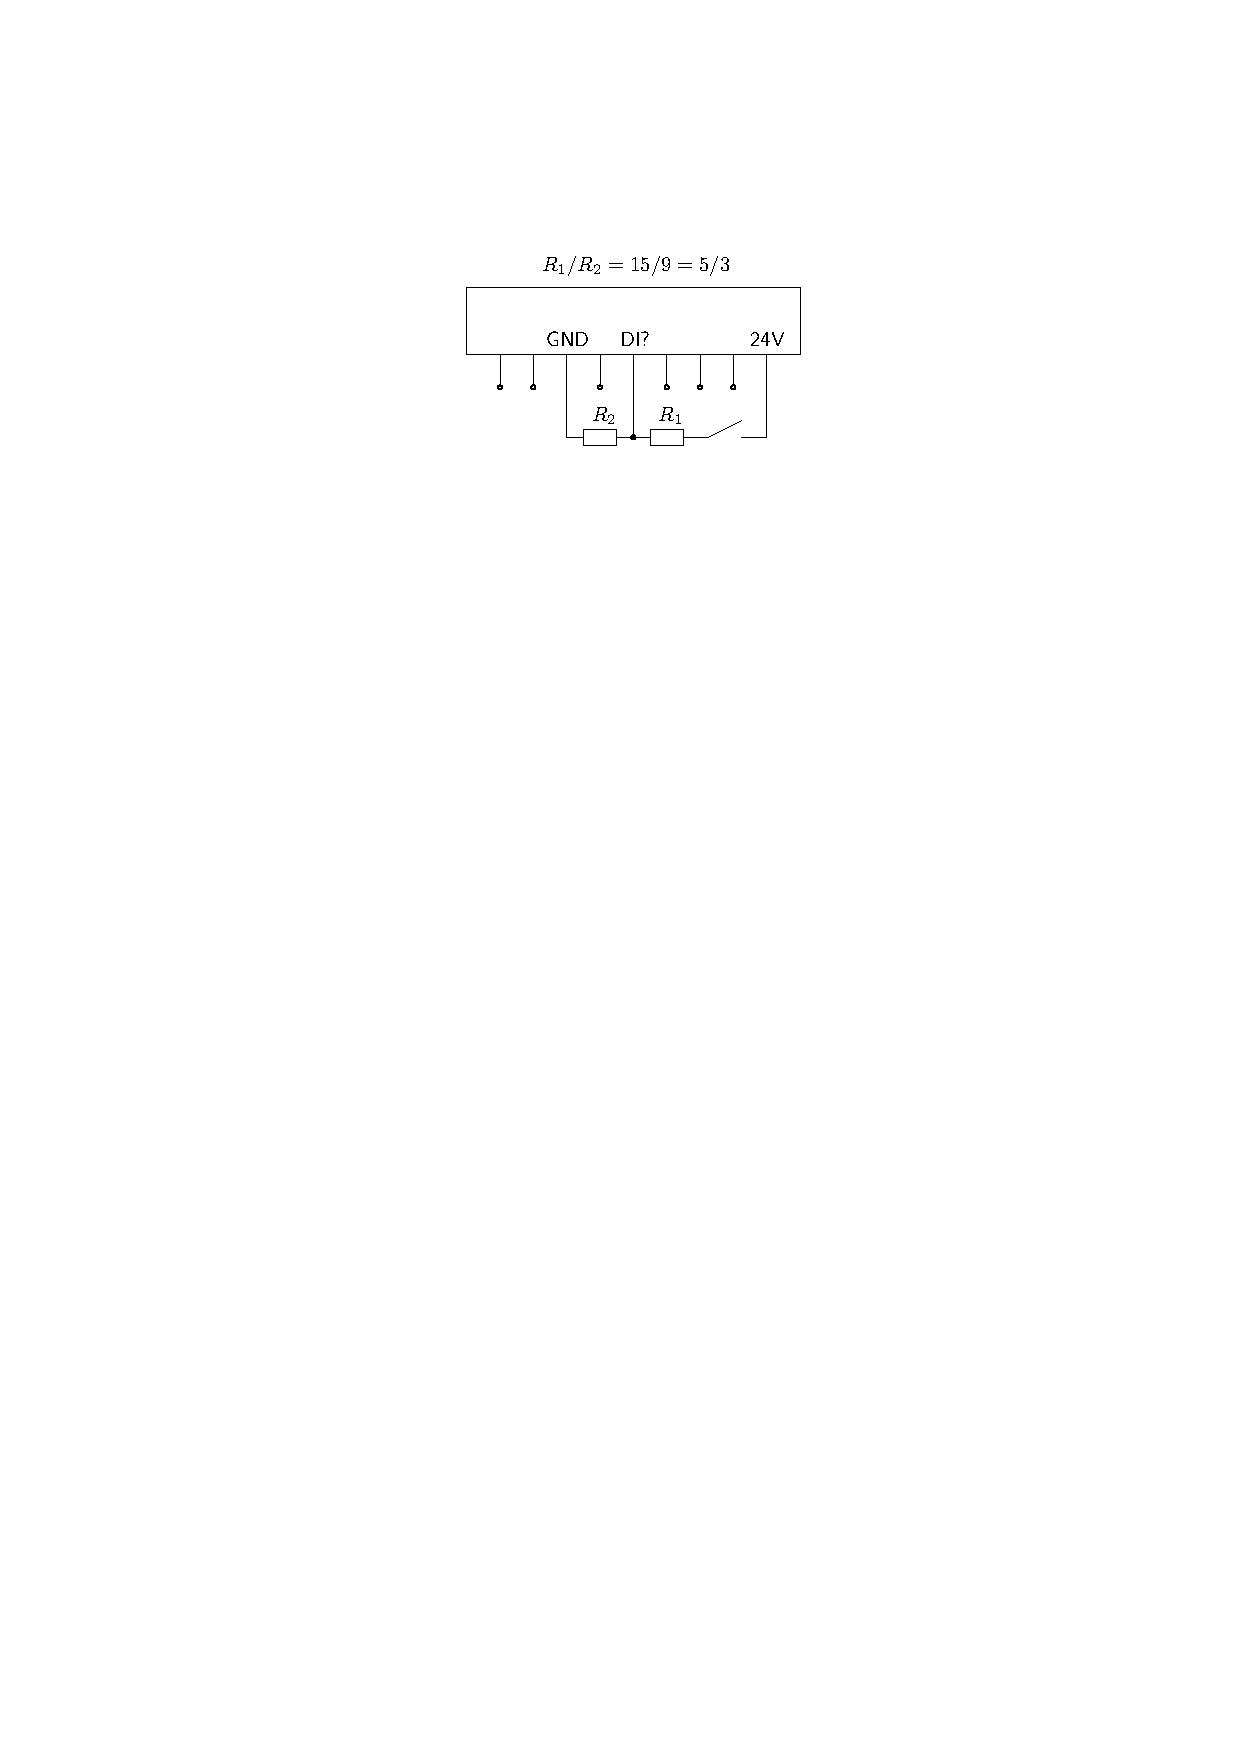
\includegraphics[width=0.6\textwidth]{button_connection.pdf}
	\caption{Схема подключения кнопок к роботу.}
	\label{img_button_connection}
\end{figure}
